\chapter{Fundamental Geometry}

\section{Fundamental 01 - Segments}

A \textbf{Segment} (đoạn thẳng) $\overline{AB}$ has finite length.

A \textbf{Line} (đường thẳng) $\overleftrightarrow{AB}$ extends out indefinitely in both directions.

A \textbf{Ray} (tia) $\overrightarrow{AB}$ only extends in one direction

A \textbf{Plane} (mặt phẳng) $ABC$. You cannot choose collinear points to notate a plane because there is an infinite number of planes that can go through that line and can be rotated.

The \textbf{intersection} of two lines is a \textbf{point} (một điểm).

The \textbf{intersection} of two planes is a line.

\textbf{Collinear points} are points that lie on the same straight line.

\textbf{Coplanar points} are points that all lie on the same plane. Any two points are always coplanar, and any three points are always coplanar, even if they are collinear (on the same line). However, four or more points are coplanar only if they all lie on the same plane

\textbf{Opposite rays} (tia đối) are two rays that share the same endpoint and extend in exactly opposite directions. Together, they form a straight line.

\newpage

\begin{figure}[ht]
  \centering
  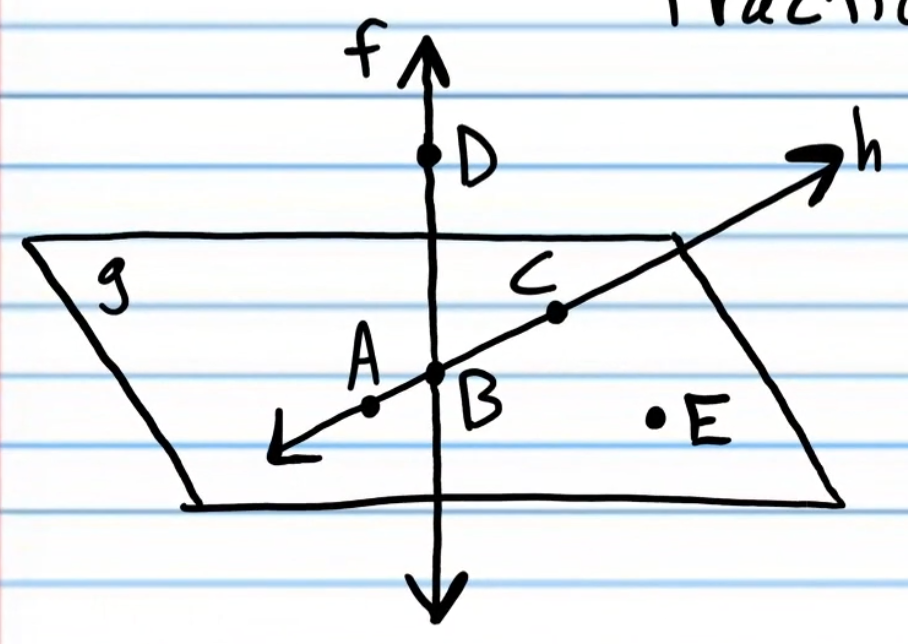
\includegraphics[width=0.5\textwidth]{0201.png}
  \caption{Bài tập}
\end{figure}

Name three collinear points on the figure above: A, B and C

Name four coplanar points: A, B, C and E

\vspace{10 mm}

\begin{figure}[ht]
  \centering
  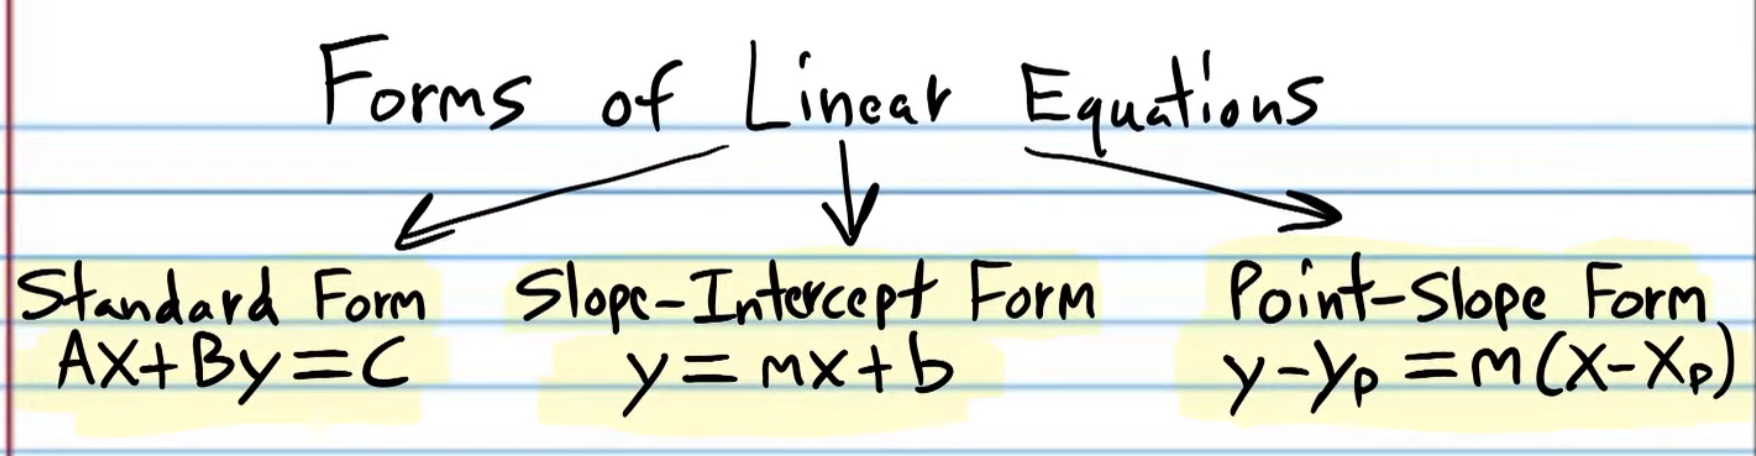
\includegraphics[width=0.5\textwidth]{0202.png}
  \caption{Bài tập}
\end{figure}

01: What is another name for FEH?

\textbf{Answer}: You can \textbf{NOT} name that plane IQK or FLE because those are collinear points. Any plane that goes through those two lines and can be rotated around is a possible plane. You have to choose three points that are not collinear.

\newpage

\begin{figure}[h!]
  \centering
  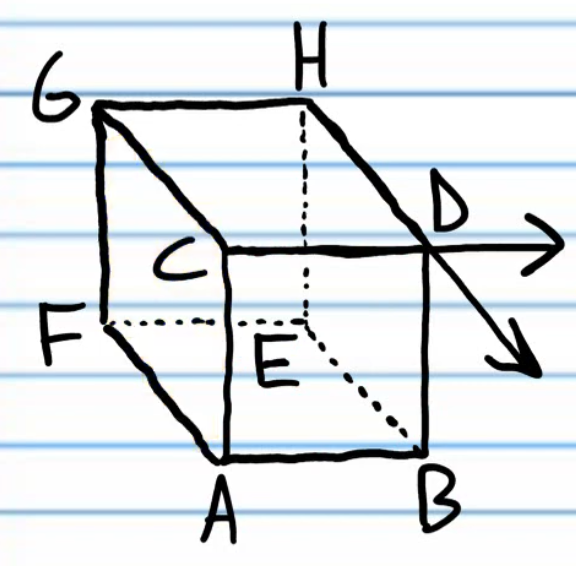
\includegraphics[width=0.5\textwidth]{0203.png}
  \caption{Bài tập}
\end{figure}

\textbf{Note}: These are planes with Finite length which means that their intersection will be segments, not lines.

01: Name three planes that intersect at B.

CAB, FEB and HDB

$\bigstar$ 02: Are F, E and A coplanar?

Any three points are always coplanar. There is at least one plane. Nếu 3 điểm colliner thì có infinite planes (you can rotate the planes).

$\bigstar$ 03: Are A and G collinear?

We don't even need to look at the picture. Any two points are collinear.

$\bigstar$ 04: Are A and H coplanar?

You can make an infinite number of planes that goes through any two points.

% \par creates a paragraph break
% \noindent prevents indentation of the current paragraph (the dot line in this case)
\par\noindent\dotfill

\textbf{Postulate} (also called an axiom): A statement that is accepted without an explanation or proof.

Theorem: A statement that requires an explanation or proof that uses definitions, postulates, other theorems, logic, etc.

\vspace{1 cm}

\centerline{\textbf{\huge Segments}}

\vspace{0.2 cm}

If $\overline{AB}$ is a segment, then AB is defined as its length (without the overline on top).

\hl{Congruence}: Having the same size and shape (notated by the symbol $\cong$). For example two triangles can be congruent.

If two segments are to be congruent, then they must have the same lengths (không cần phải cùng hướng hay song song gì cả).

Example: If $\overline{AB} \cong \overline{CD}$, then AB=CD.

\begin{tcolorbox}[colback=blue!5!white,colframe=blue!75!black,title=The Segmennt Addition Postulate]
  If A, B, and C are collinear, and B is between A and C, then $AB + BC = AC$.
\end{tcolorbox}

\begin{figure}[h]
  \centering
  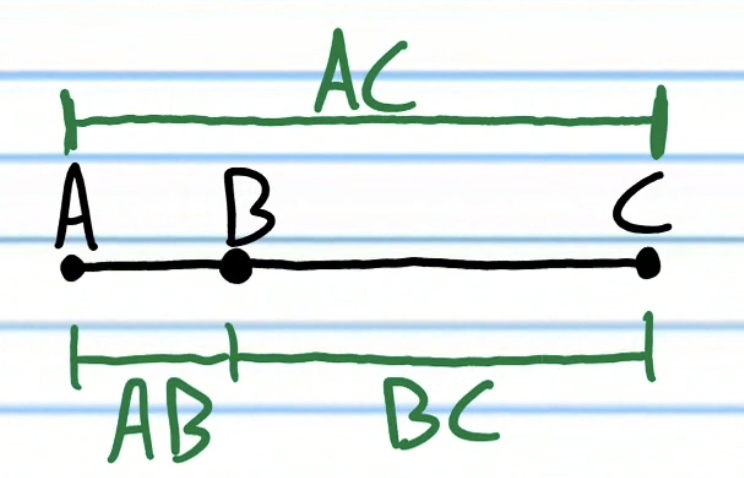
\includegraphics[width=0.4\textwidth]{0204.png}
  \caption{The Segment Addition Postulate}
\end{figure}

\hl{Midpoint of a Segment}: A point (e.g. M below) that is in the middle or center of a segment, dividing it into two congruent segments.

\begin{figure}[h]
  \centering
  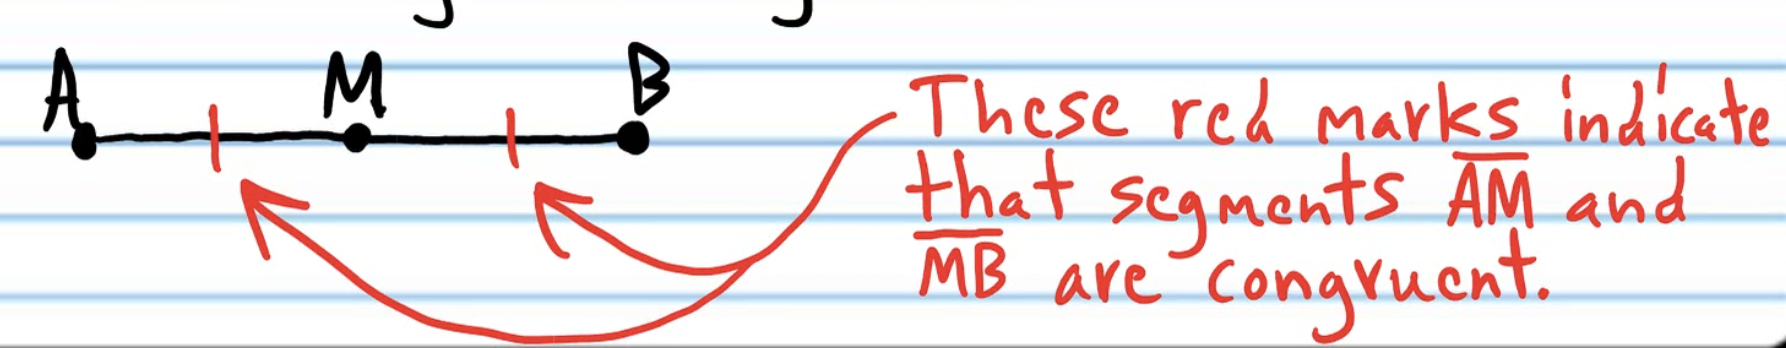
\includegraphics[width=0.7\textwidth]{0205.png}
  \caption{Midpoint of a Segment}
\end{figure}

\hl{Bisect}: (verb) To divide into two \textbf{equal} parts.

\hl{Segment Bisector}: A point, ray, line, segment or plane that divides a segment into two congruent segments by intersecting at its midpoint.

\begin{figure}[htb!]
  \centering
  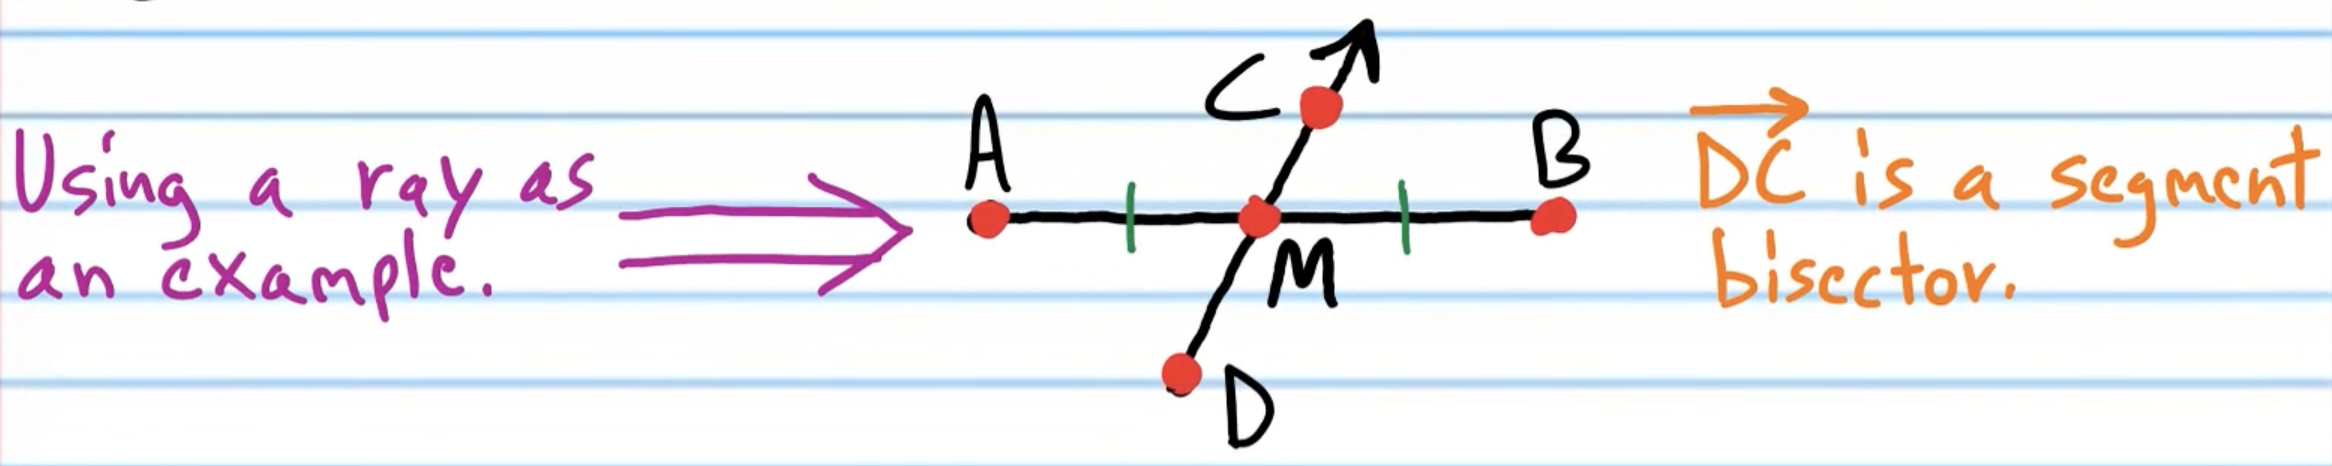
\includegraphics[width=0.7\textwidth]{0206.png}
  \caption{Segment Bisector}
\end{figure}

\section{Fundamental 02 - Angles}

\hl{Angle}: Two \textbf{rays} with a common \textbf{endpoint} that help to indicate a measure of rotation.

\begin{figure}[htb!]
  \centering
  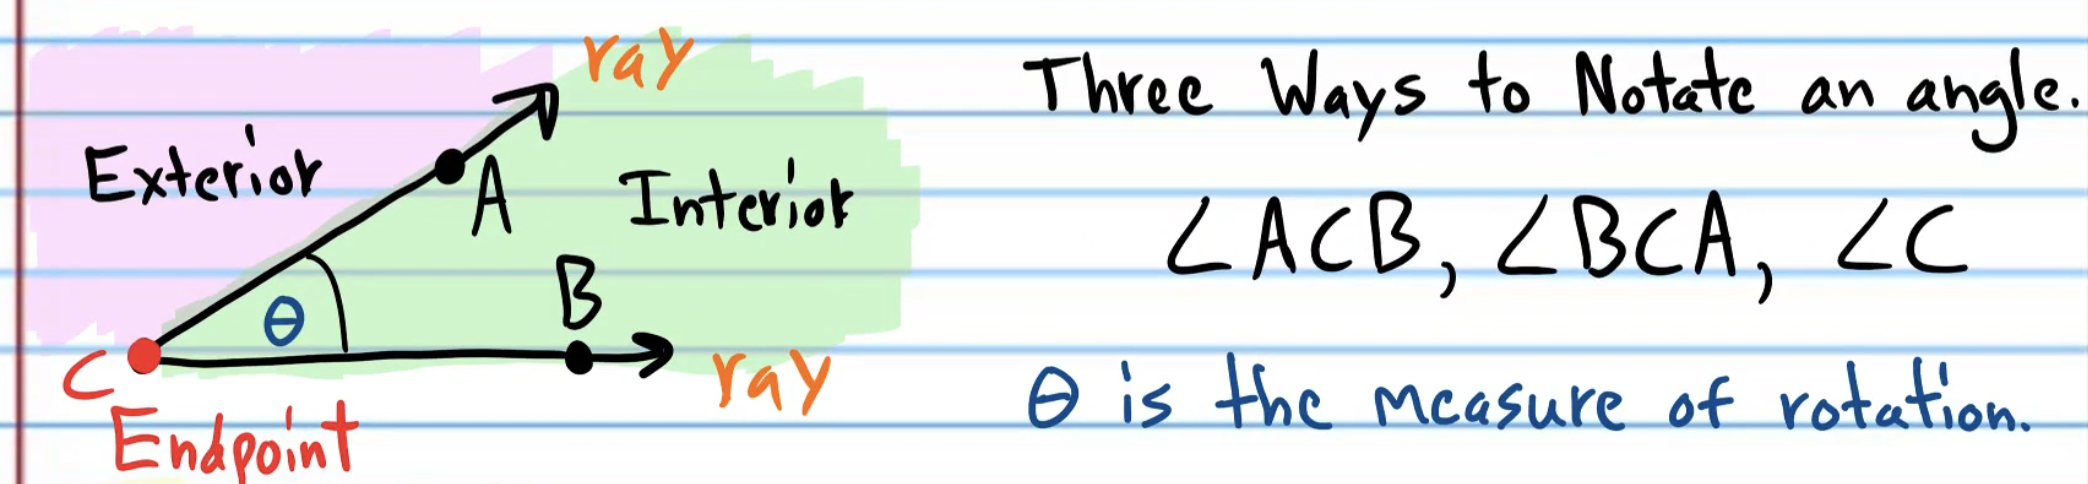
\includegraphics[width=0.7\textwidth]{0301.png}
  \caption{An Angle}
\end{figure}

\hl{Angle Vertex}: The common \textbf{endpoint} of the two \textbf{rays}.

\hl{Angle Sides}: The two \textbf{rays}.

$\angle ABC$ refer to the concept of the angle. You can write a letter m in front like $m\angle ABC$ to represents the \textbf{measure} of the angle (which is just a number). Or you can also use a Greek letter (e.g. $\theta$).

\vspace{1 cm}

\centerline{\textbf{\huge Classifying Angles}}

\vspace{0.2 cm}

\hl{Right Angle} góc vuông $90^{\circ}$

\hl{Acute angle} (Góc nhọn): $0^{\circ} < \Theta < 90^{\circ}$

\hl{Straight Angle} góc bẹt $180^{\circ}$

\hl{Obtuse angle} (Góc tù) $90^{\circ} < \Theta < 180^{\circ}$

\hl{Reflex angle} (Góc lõm) $180^{\circ} < \Theta < 360^{\circ}$

\hl{Full angle, rotation angle} $\Theta = 360^{\circ}$

\newpage

Angle Addition Postulate. A postulate is what we accept to be true without requiring any explanation.

\begin{figure}[htb!]
  \centering
  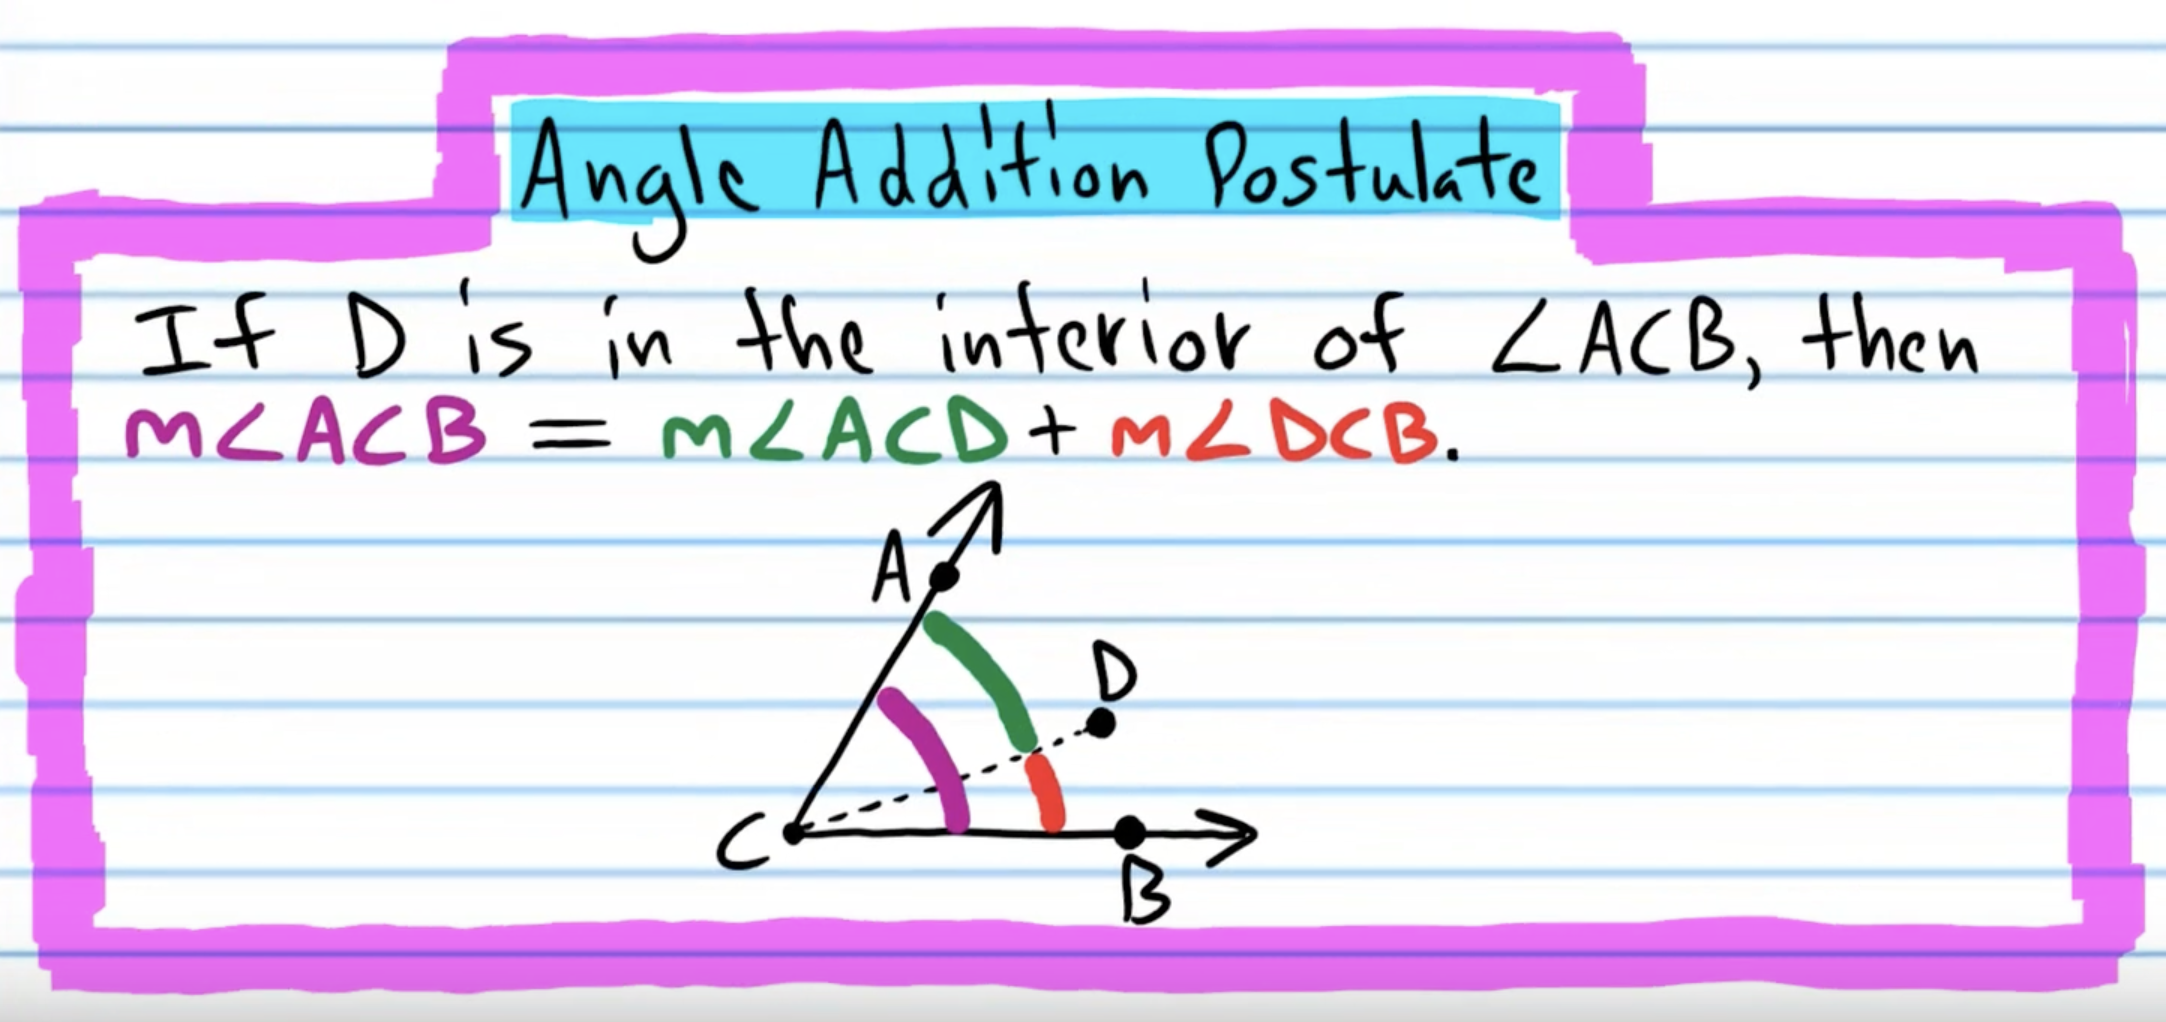
\includegraphics[width=0.7\textwidth]{0302.png}
  \caption{Angle Addition Postulate}
\end{figure}

If two angles are \textbf{congruent}, then their measures are equal. We write $\angle ABD \cong \angle DBC$ but $m\angle ABD = m\angle DBC$.

\hl{Angle Bisector}: A \textbf{ray} that divides an angle in half, such that the two resulting angles are congruent.

\vspace{0.9 cm}

\centerline{\textbf{\huge Angle Pairs}}

\vspace{0.2 cm}

\hl{Adjacent Angles}: Two angles that share a vertex and a side but have no common interior points.

\begin{figure}[htb!]
  \centering
  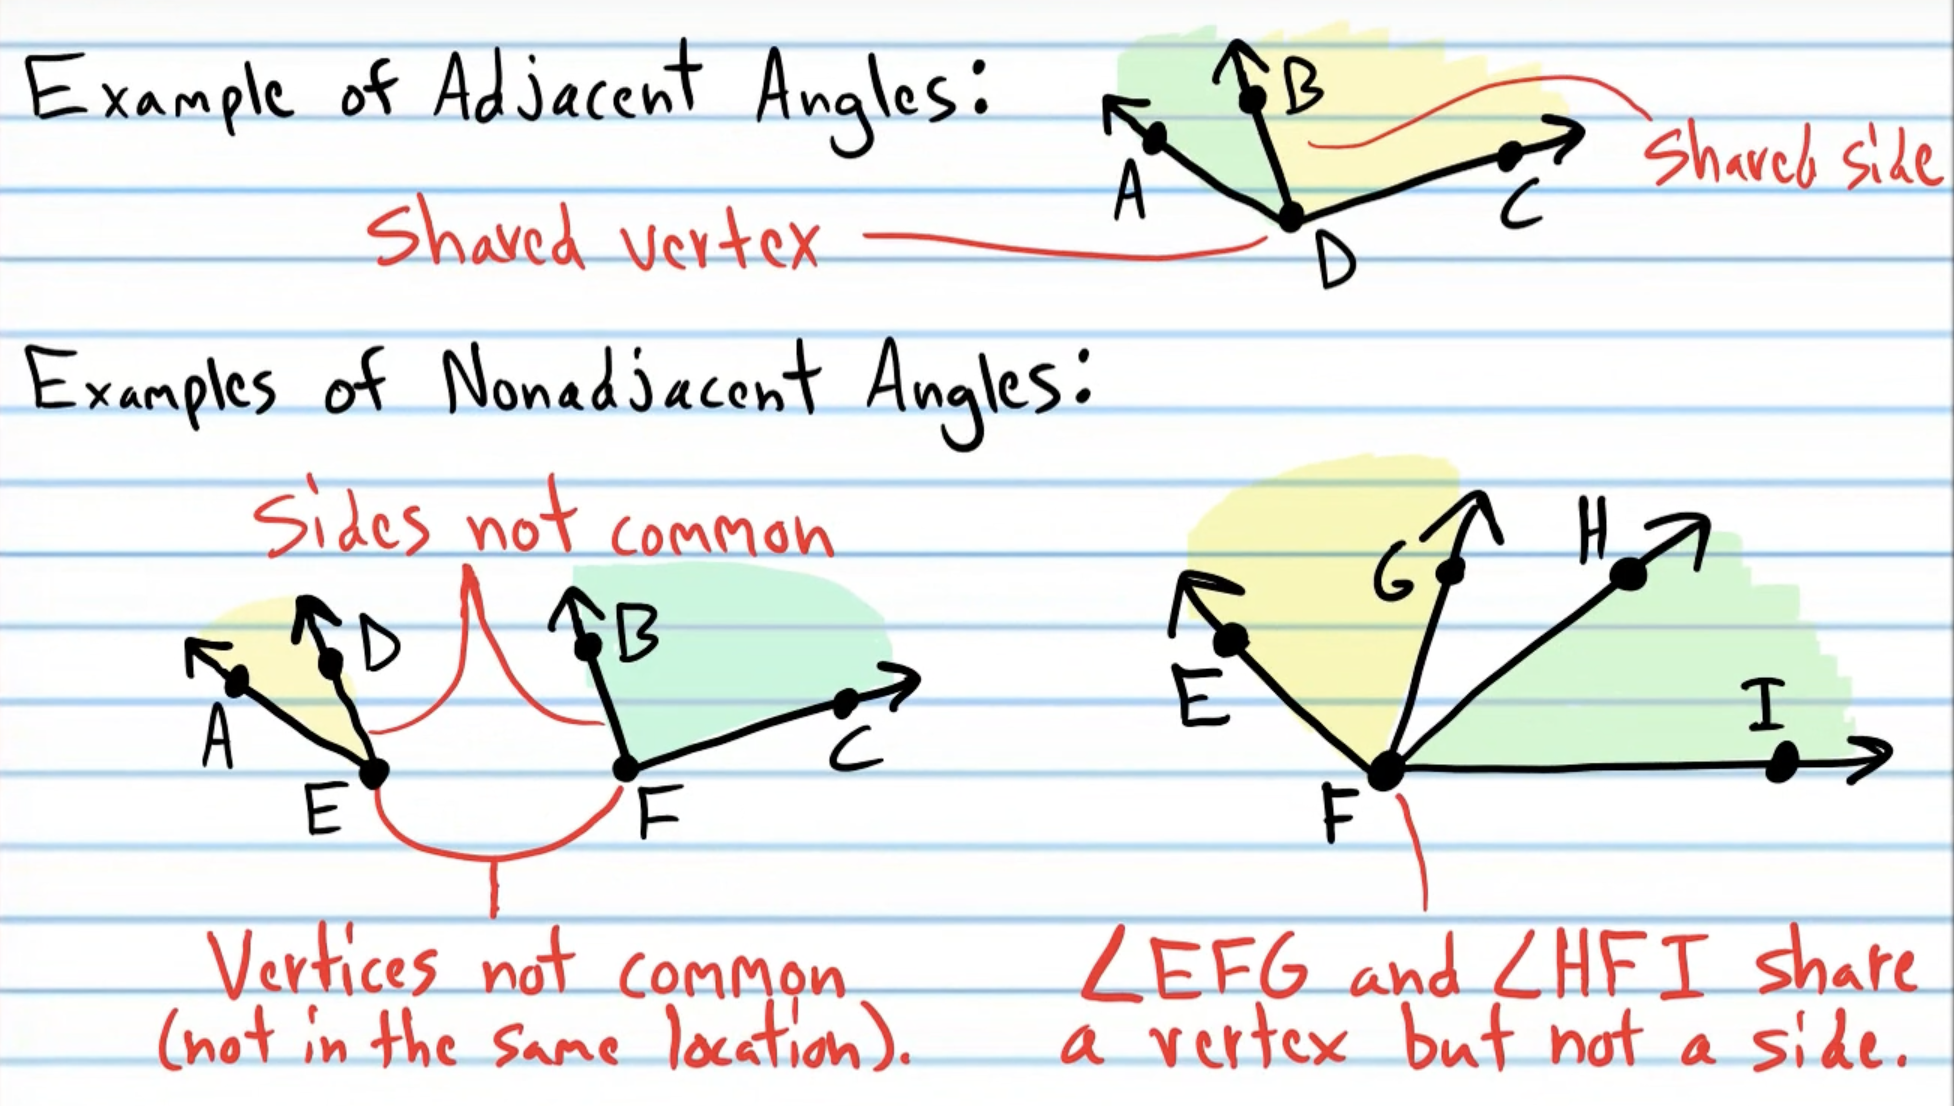
\includegraphics[width=0.8\textwidth]{0303.png}
  \caption{Adjacent Angles}
\end{figure}

\newpage

\hl{Complementary Angles}: Two angles whose measures add up to $90^{\circ}$.

\begin{figure}[htb!]
  \centering
  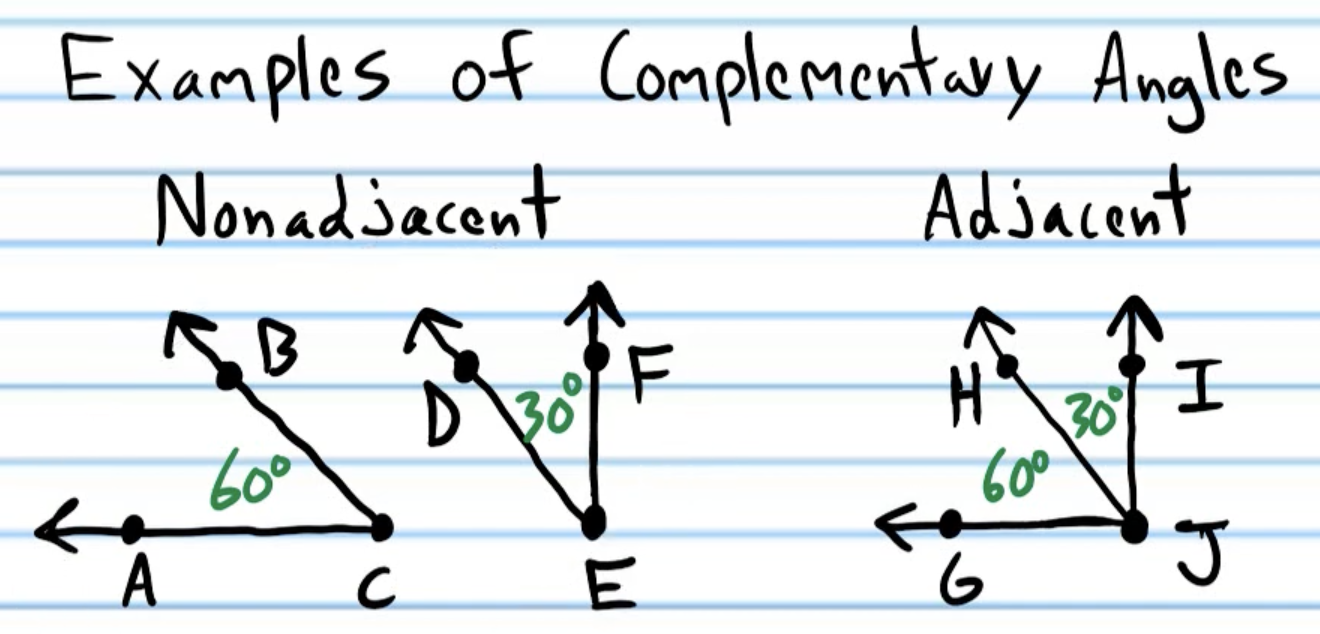
\includegraphics[width=0.7\textwidth]{0304.png}
  \caption{Complementary Angles}
\end{figure}

Compliment spelled with an \q{i} is a comment that expresses praise or approval of somebody. But Complement with an \q{e} means you make something better by adding something to it.

Remember the \q{c} in complement => Chín chục.

\vspace{10 mm}

\hl{Supplementary Angles}: Two angles whose measures add up to $180^{\circ}$.

\begin{figure}[htb!]
  \centering
  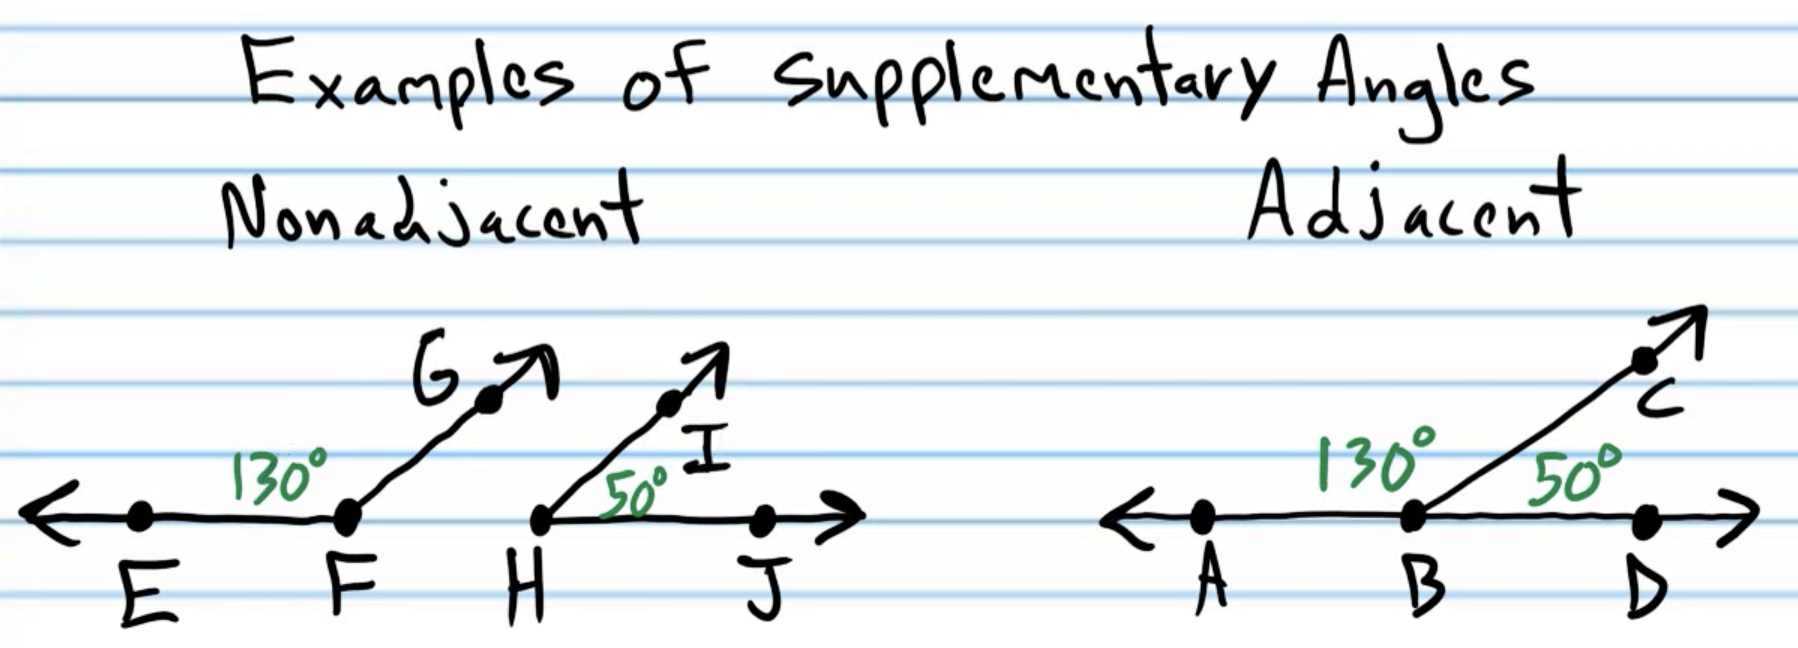
\includegraphics[width=0.7\textwidth]{0305.png}
  \caption{Supplementary Angles}
\end{figure}

\textbf{Bai tập 25}: If the measure of an angle is $40^{\circ}$ less than the measure of its supplement, what is the measure of the angle?

\vspace{0.2 cm}

\centerline{\textbf{\normalsize Answer}}

\vspace{0.2 cm}

Giải system of equation below bằng substitution:

\begin{equation*}
    \begin{cases}
      m\angle A + m\angle B = 180\\
      m\angle A = m\angle B -40
    \end{cases}\,.
\end{equation*}

\vspace{5 cm}

\hl{Linear Pair} (cặp góc kề bù): Two adjacent angles whose non-common sides are opposite rays.

\begin{figure}[htb!]
  \centering
  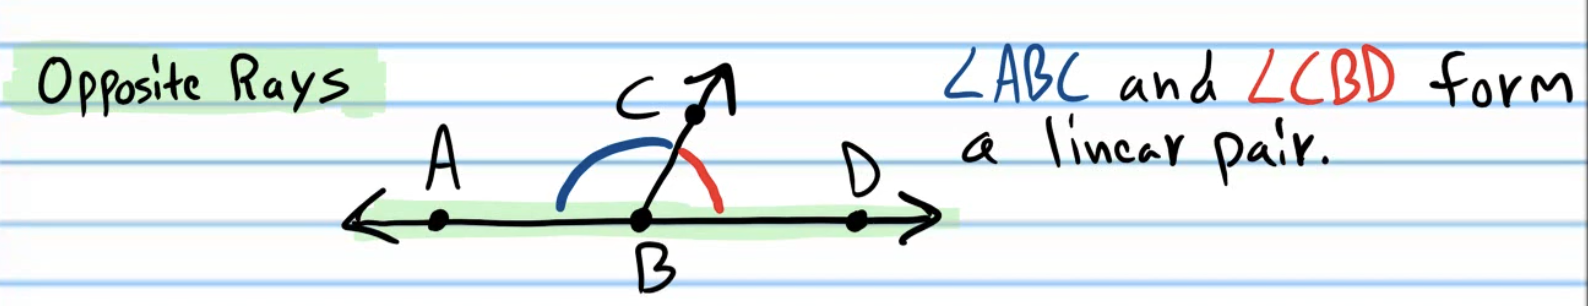
\includegraphics[width=0.8\textwidth]{0306.png}
  \caption{Linear Pair}
\end{figure}

% \colorbox{SkyBlue}{Linear Pair Postulate}: If two angles from a linear pair, they are supplementary.

\begin{tcolorbox}[colback=RoyalPurple!5!white,colframe=RoyalPurple!75!black]
  \colorbox{SkyBlue}{Linear Pair Postulate}: If two angles from a linear pair, they are supplementary.
\end{tcolorbox}

\vspace{1 cm}

\hl{Vertical Angles} (or opposite angles): Two angles whose sides form two pairs of opposite rays. Or when two lines intersect.

\begin{figure}[htb!]
  \centering
  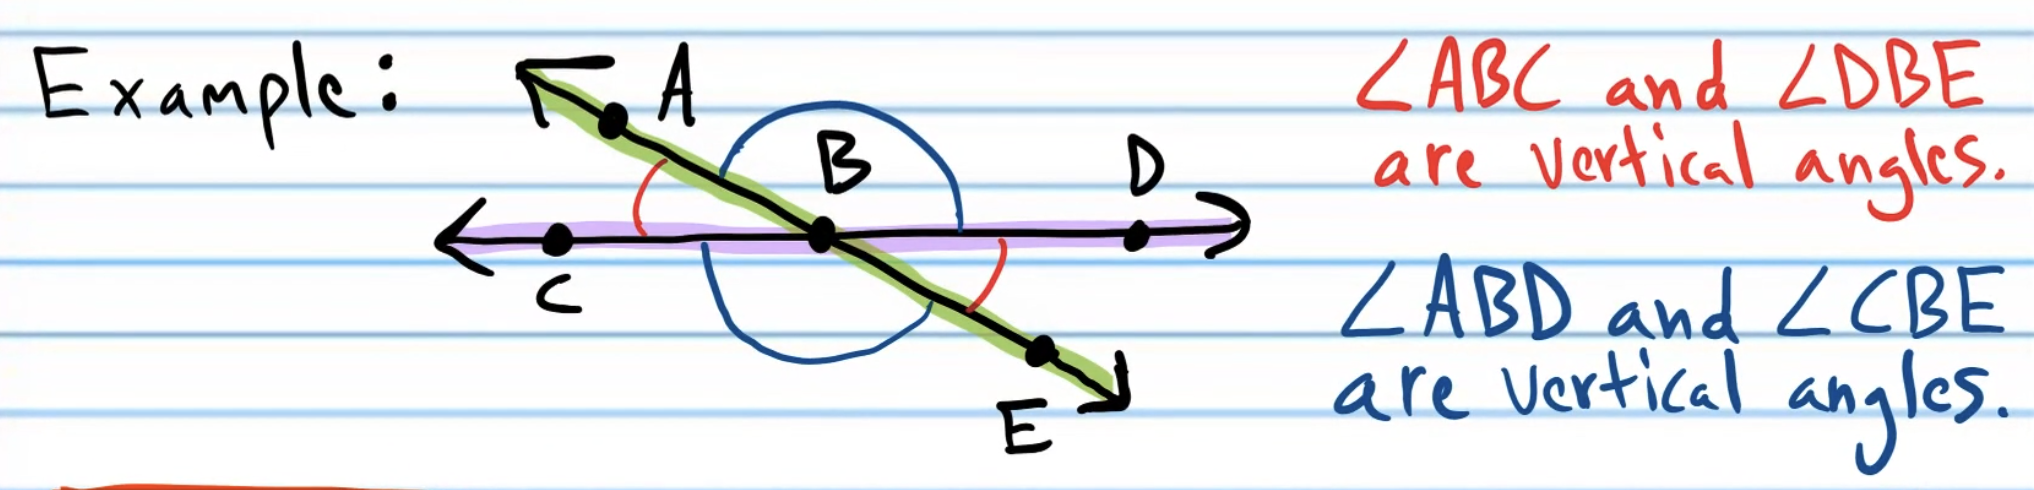
\includegraphics[width=0.8\textwidth]{0307.png}
  \caption{Vertical Angles}
\end{figure}

\begin{tcolorbox}[colback=red!5!white,colframe=red!75!black,title=Vertical Angles Theorem]
  Vertical angles are congruent.
\end{tcolorbox}

This is the first theorem that we learn. We will not prove it now. Unlike postulates, theorems need to be proven.

When doing proofs, you can skip right to saying that the measures of the two angles are equal to each other.

\section{Fundamental 03 - Polygons}

\newpage

\hl{Polygon}: A closed plane figure whose sides are segments that intersects only at endpoints.

\begin{figure}[htb!]
  \centering
  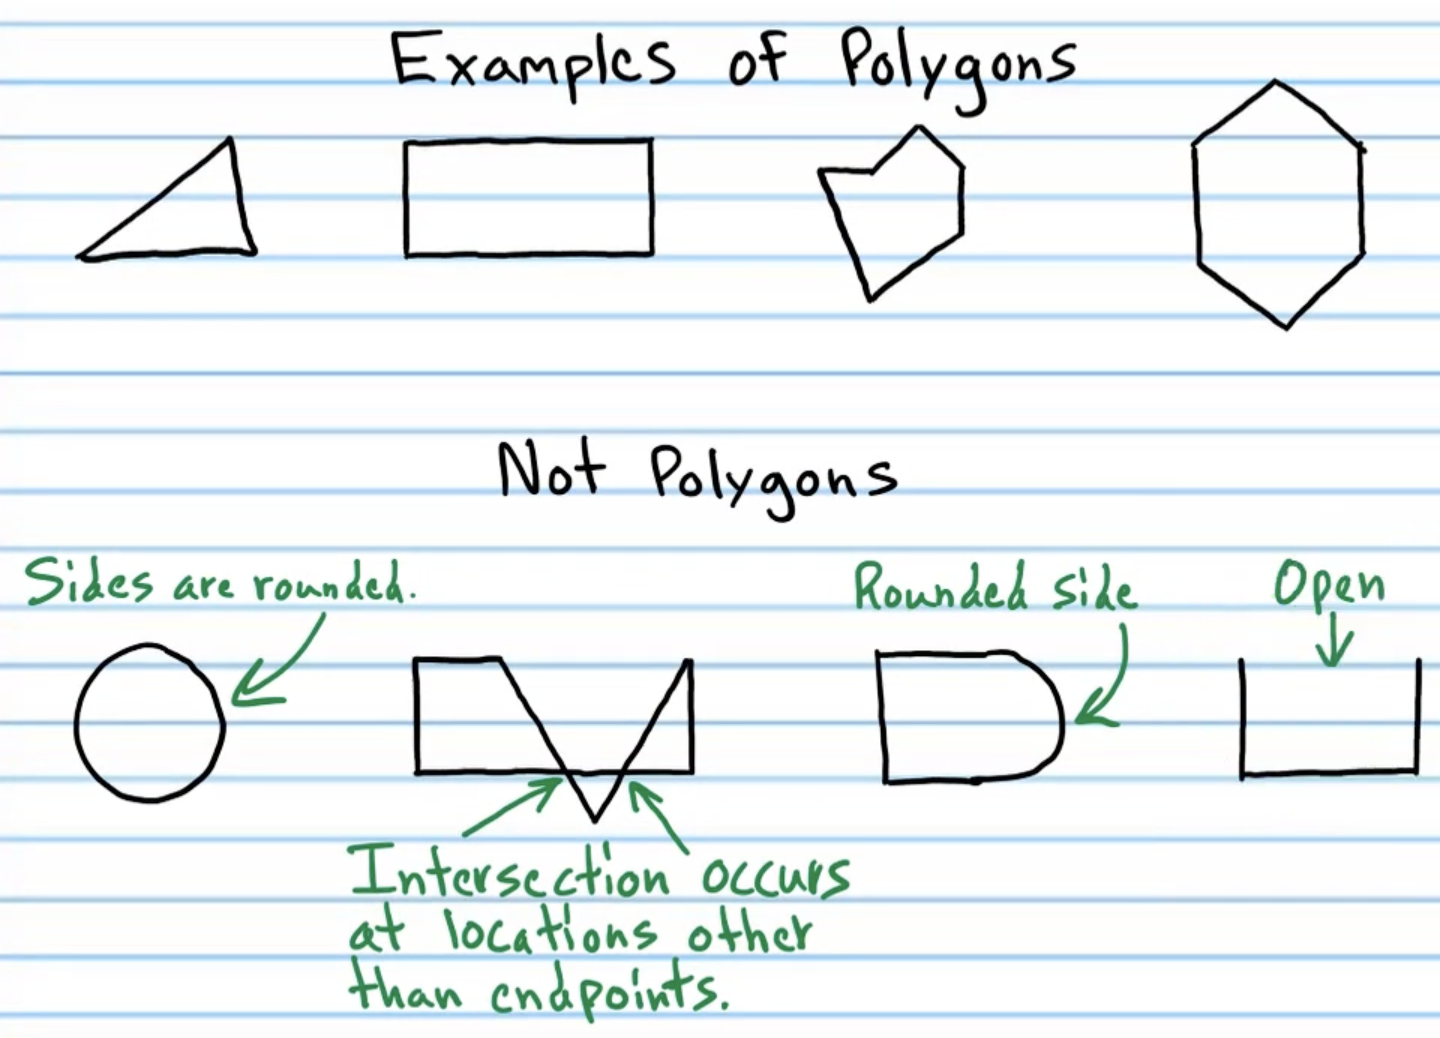
\includegraphics[width=0.8\textwidth]{0401.png}
  \caption{Polygons}
\end{figure}

Parts of a Polygon.

\begin{figure}[htb!]
  \centering
  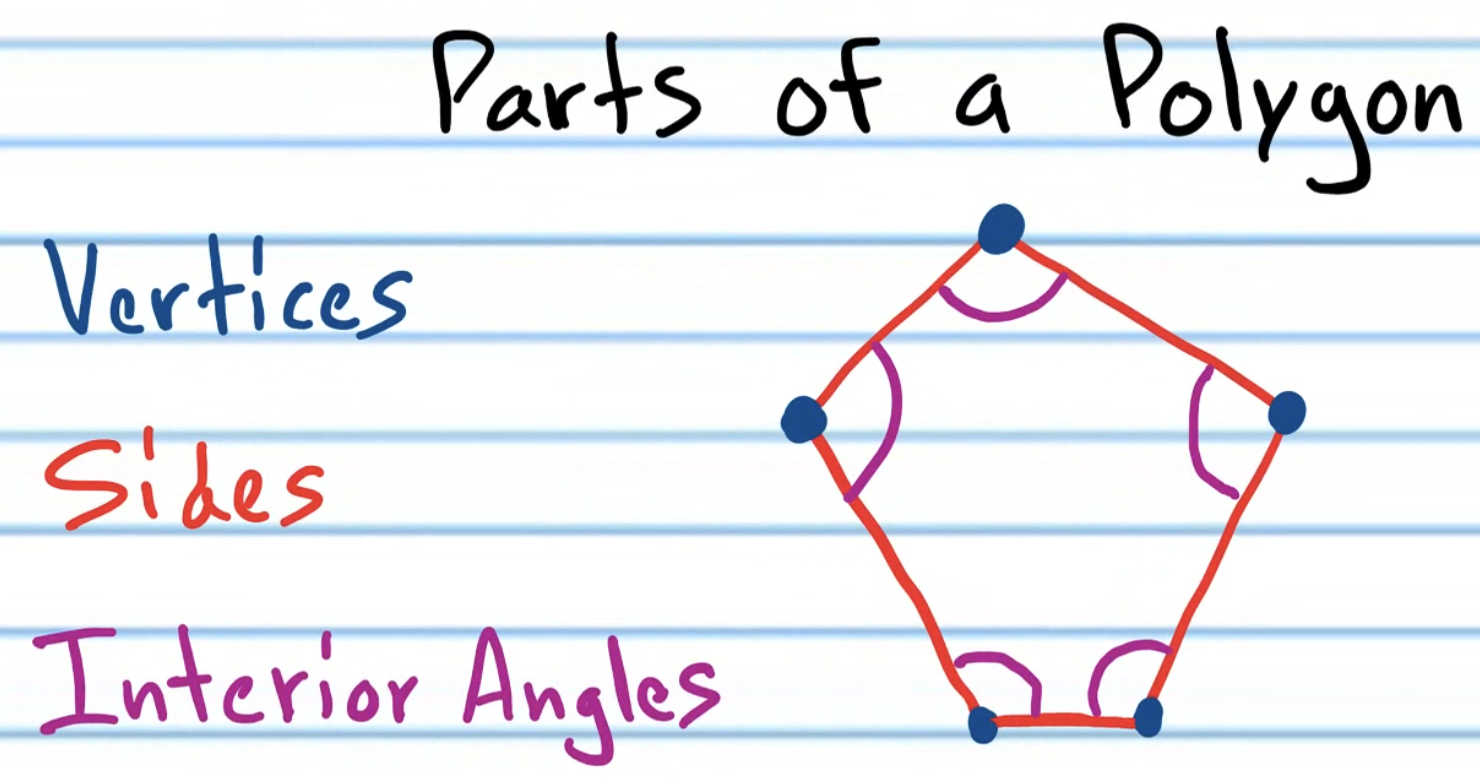
\includegraphics[width=0.7\textwidth]{0402.png}
  \caption{Parts of a Polygons}
\end{figure}

\newpage

Names of Polygons. Number of sides = number of angles.

\begin{center}
\begin{tabular}{ c | c }
  \textbf{Sides} & \textbf{Name} \\
  \hline
  3 & Triangle \\
  4 & Quadrilateral, tứ giác \\
  5 & Pentagon \\
  6 & Hexagon \\
  7 & Heptaton, Septaton \\
  8 & Octagon \\
  9 & Nonagon \\
  10 & Decagon \\
  12 & Dodecagon \\
  n & n-gon \\
\end{tabular}
\end{center}

\begin{figure}[htb!]
  \centering
  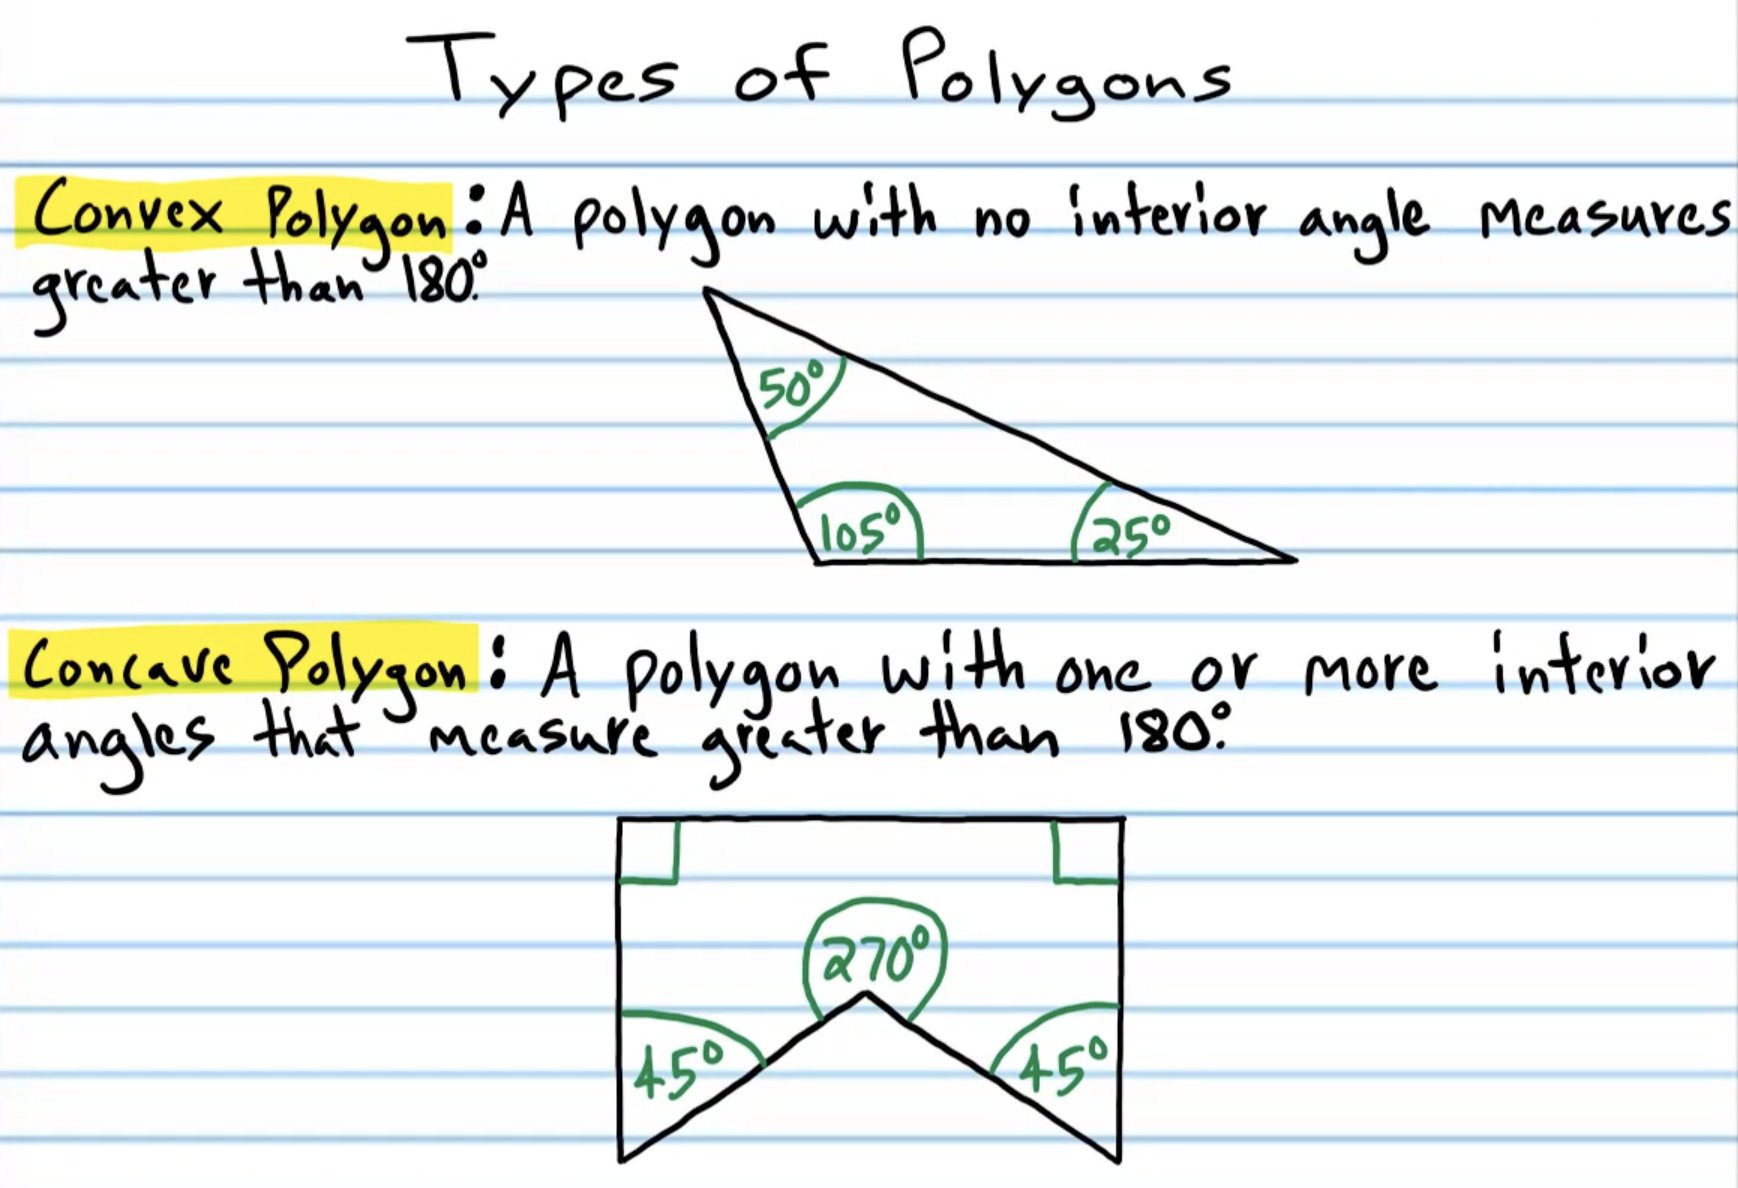
\includegraphics[width=0.8\textwidth]{0403.png}
  \caption{Types of Polygons}
\end{figure}

Convex: curving out; concave is curving in (bị lõm).

\vspace{1cm}

\newpage

More types of Polygons. Tránh nhầm equilateral vs quadrilateral (tứ giác).

\begin{figure}[htb!]
  \centering
  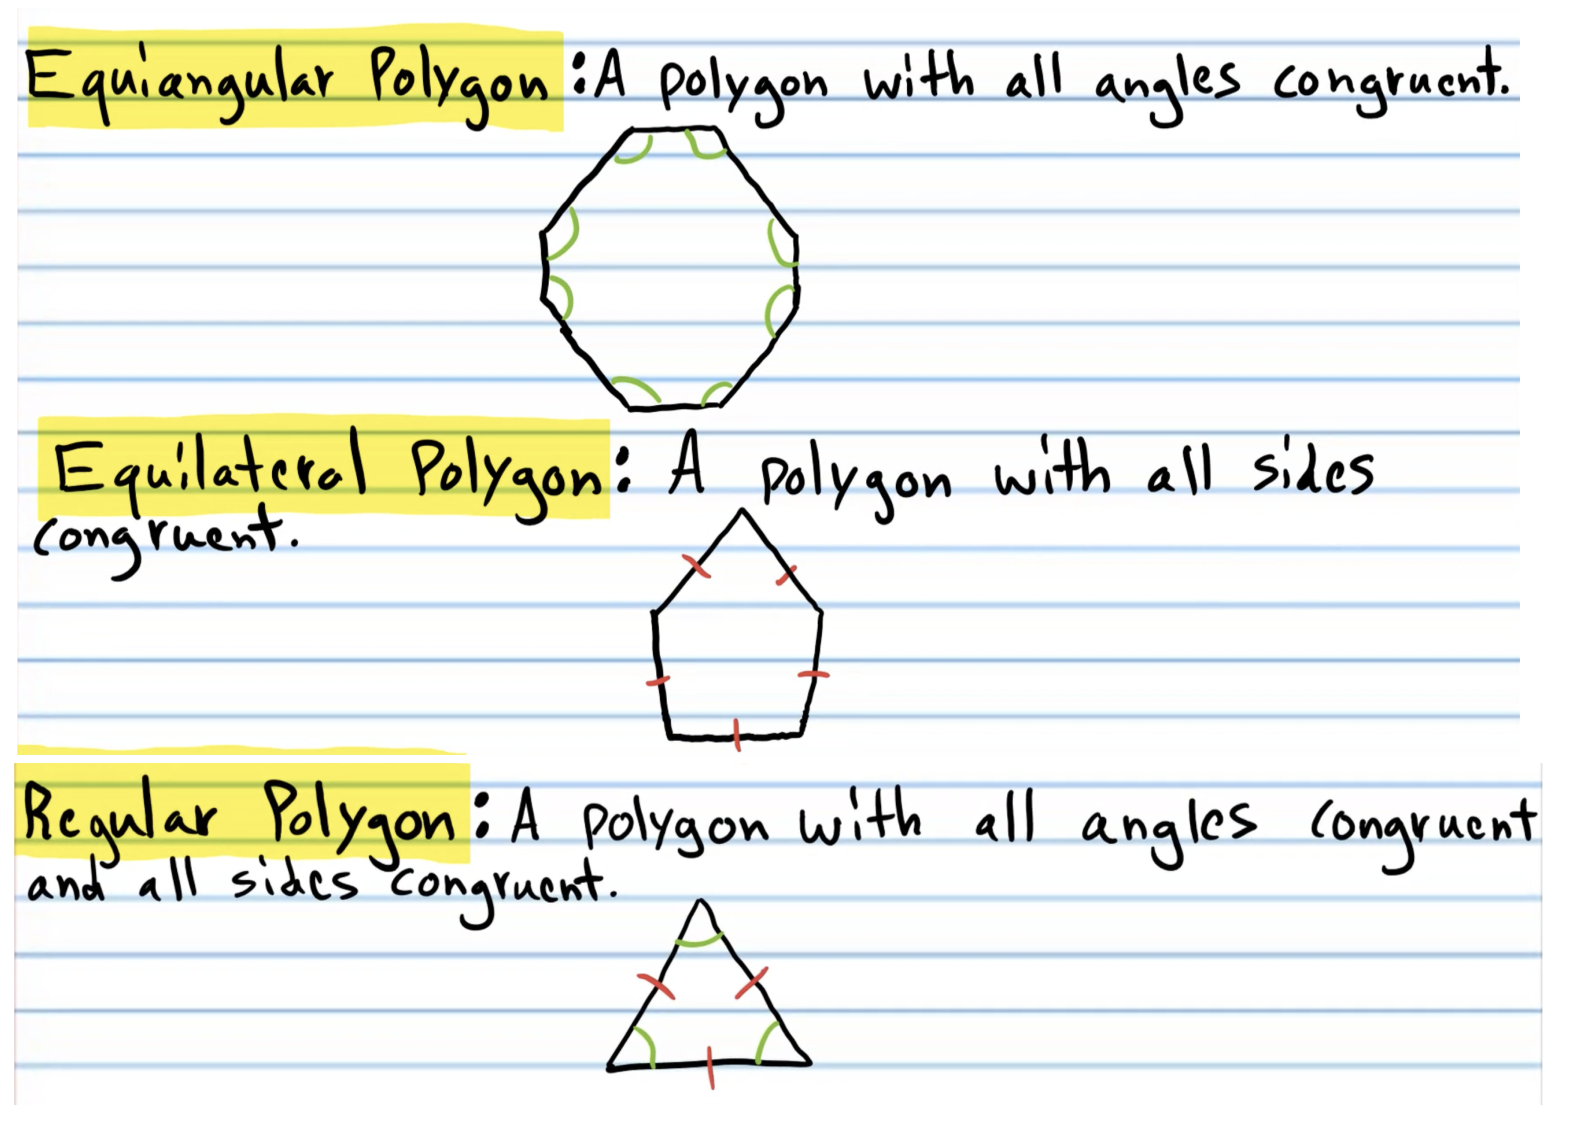
\includegraphics[width=0.8\textwidth]{0404.png}
  \caption{Equiangular, Equilateral, and Regular Polygon}
\end{figure}

Two polygons are the same size and shape if and only if they are \textbf{congruent}.

\vspace{0.6 cm}

\centerline{\textbf{\huge Geometric Formulas}}

\vspace{0.2 cm}

Perimeter (chu vi) of a Rectangle or Square: \colorbox{ForestGreen}{$P=2L+2W$}

Area of a Rectangle or Square: \colorbox{pink}{$A=LW$}

Area of a Triangle: \colorbox{red}{$A=\frac{bh}{2}$}

Volume of a Rectangular Prism (Hình hộp chữ nhật): \colorbox{cyan}{$V=LWH$}

Surface Area of a Rectangular Prism: \colorbox{yellow}{$A=2LW+2LH+2WH$}

Diameter of a Circle: \colorbox{brown}{$D=2r$}

Area of a Parallelogram (Hình bình hành): \colorbox{green}{$A=bh$}

Perimeter of a circle (i.e. circumference): \colorbox{VioletRed}{$C=2\pi r$} or \colorbox{VioletRed}{$\pi D$}.

Area of a Circle: \colorbox{orange}{$A=\pi r^{2}$}

Volume of a Sphere: \colorbox{pink}{$V=\frac{4\pi r^{3}}{3}$}

Surface Area of a Sphere: \colorbox{BlueGreen}{$A=4\pi r^{2}$}

Volume of a Cylinder: \colorbox{green}{$V=\pi r^{2}h$}

Volume of a Cone: \colorbox{red}{$V=\frac{\pi r^{2}h}{3}$}

Area of a Trapezoid (hình thang): \colorbox{LimeGreen}{$A=\frac{h(b_{1}+b_{2})}{2}$}

\section{Proofs and Properties of Equality and Congruence}
% 20 Aug 2025

Most of this section is written in the Algebra Notes. Here, we will only cover some geometric-specific concepts that are necessary for the proofs.

\hl{Perpendicular Lines}: Lines that intersect to form right angles. The symbol for perpendicular lines is $\overline{AB} \perp \overline{CD}$.

\vspace{.5cm}

\begin{tcolorbox}[colback=red!5!white,colframe=red!75!black,title=Right Angle Congruence Theorem]
  If two angles are both right angles, then they are congruent. 
\end{tcolorbox}

This theorem might seem obvious, but it will allow us to skip steps when doing other proofs.

\vspace{.5cm}

\begin{tcolorbox}[colback=OrangeRed!5!white,colframe=OrangeRed!75!black,title=Congruent Supplements Theorem]
  If two angles are supplementary to the same angle, then they are congruent.
\end{tcolorbox}

\vspace{.3cm}

\begin{tcolorbox}[colback=Orange!5!white,colframe=Orange!75!black,title=Congruent Complements Theorem]
  If two angles are complementary to the same angle, then they are congruent.
\end{tcolorbox}

\newpage

\section{Angles Formed by Transversals}
% 28 Sep 2025, after studying beginning algebra for quite a while, I am back!
% Mới đám giỗ yesterday. Always rain the sky recently.

\hl{Tranversal} is a line that goes through two or more other lines.

\begin{figure}[htb!]
  \centering
  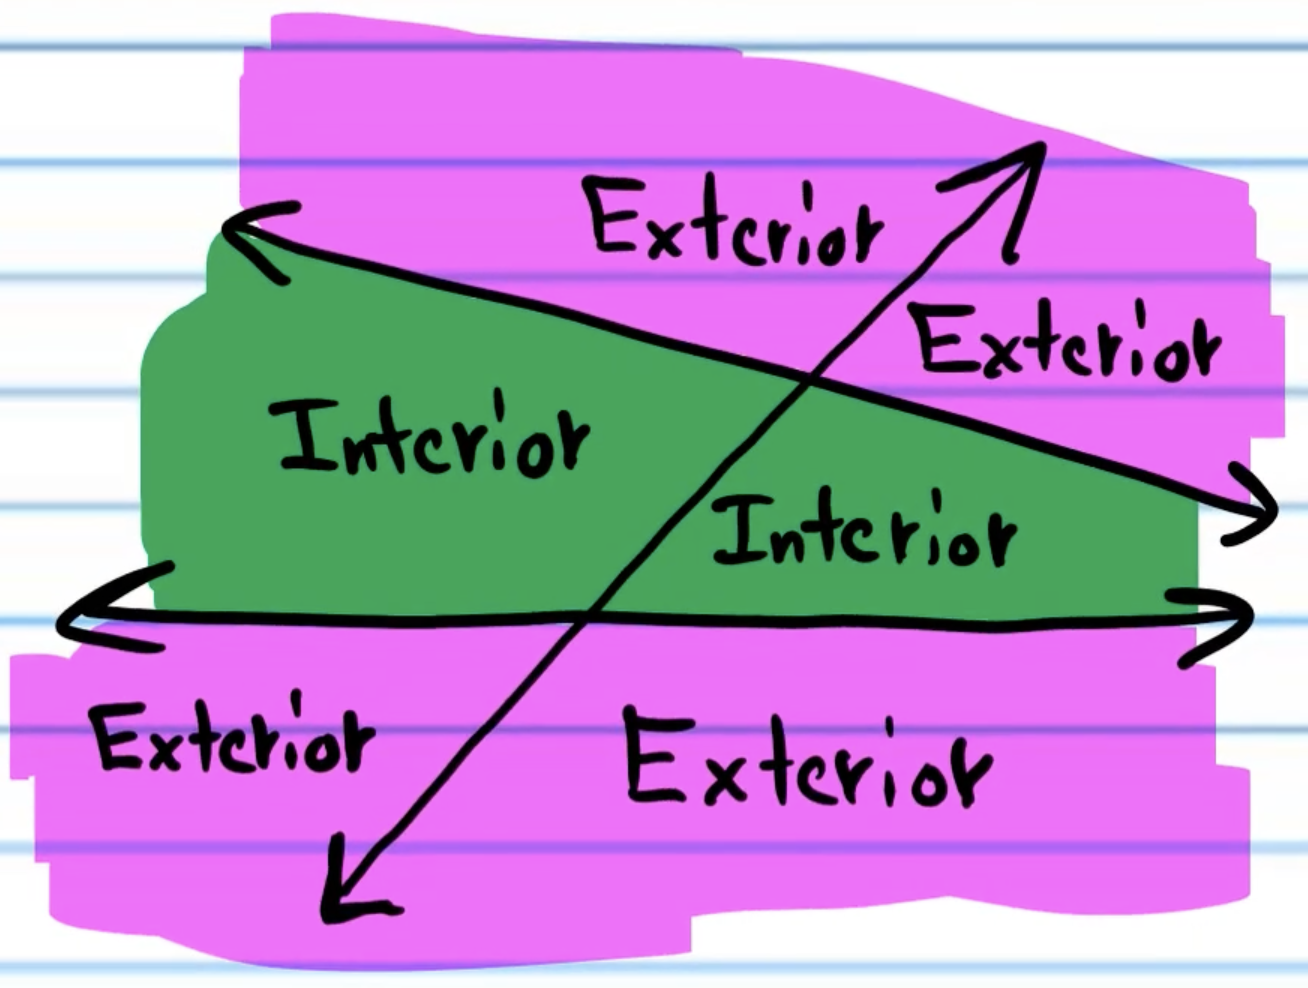
\includegraphics[width=0.7\textwidth]{1101.png}
  \caption{Angles Formed by Transversals}
\end{figure}

\begin{figure}[htb!]
  \centering
  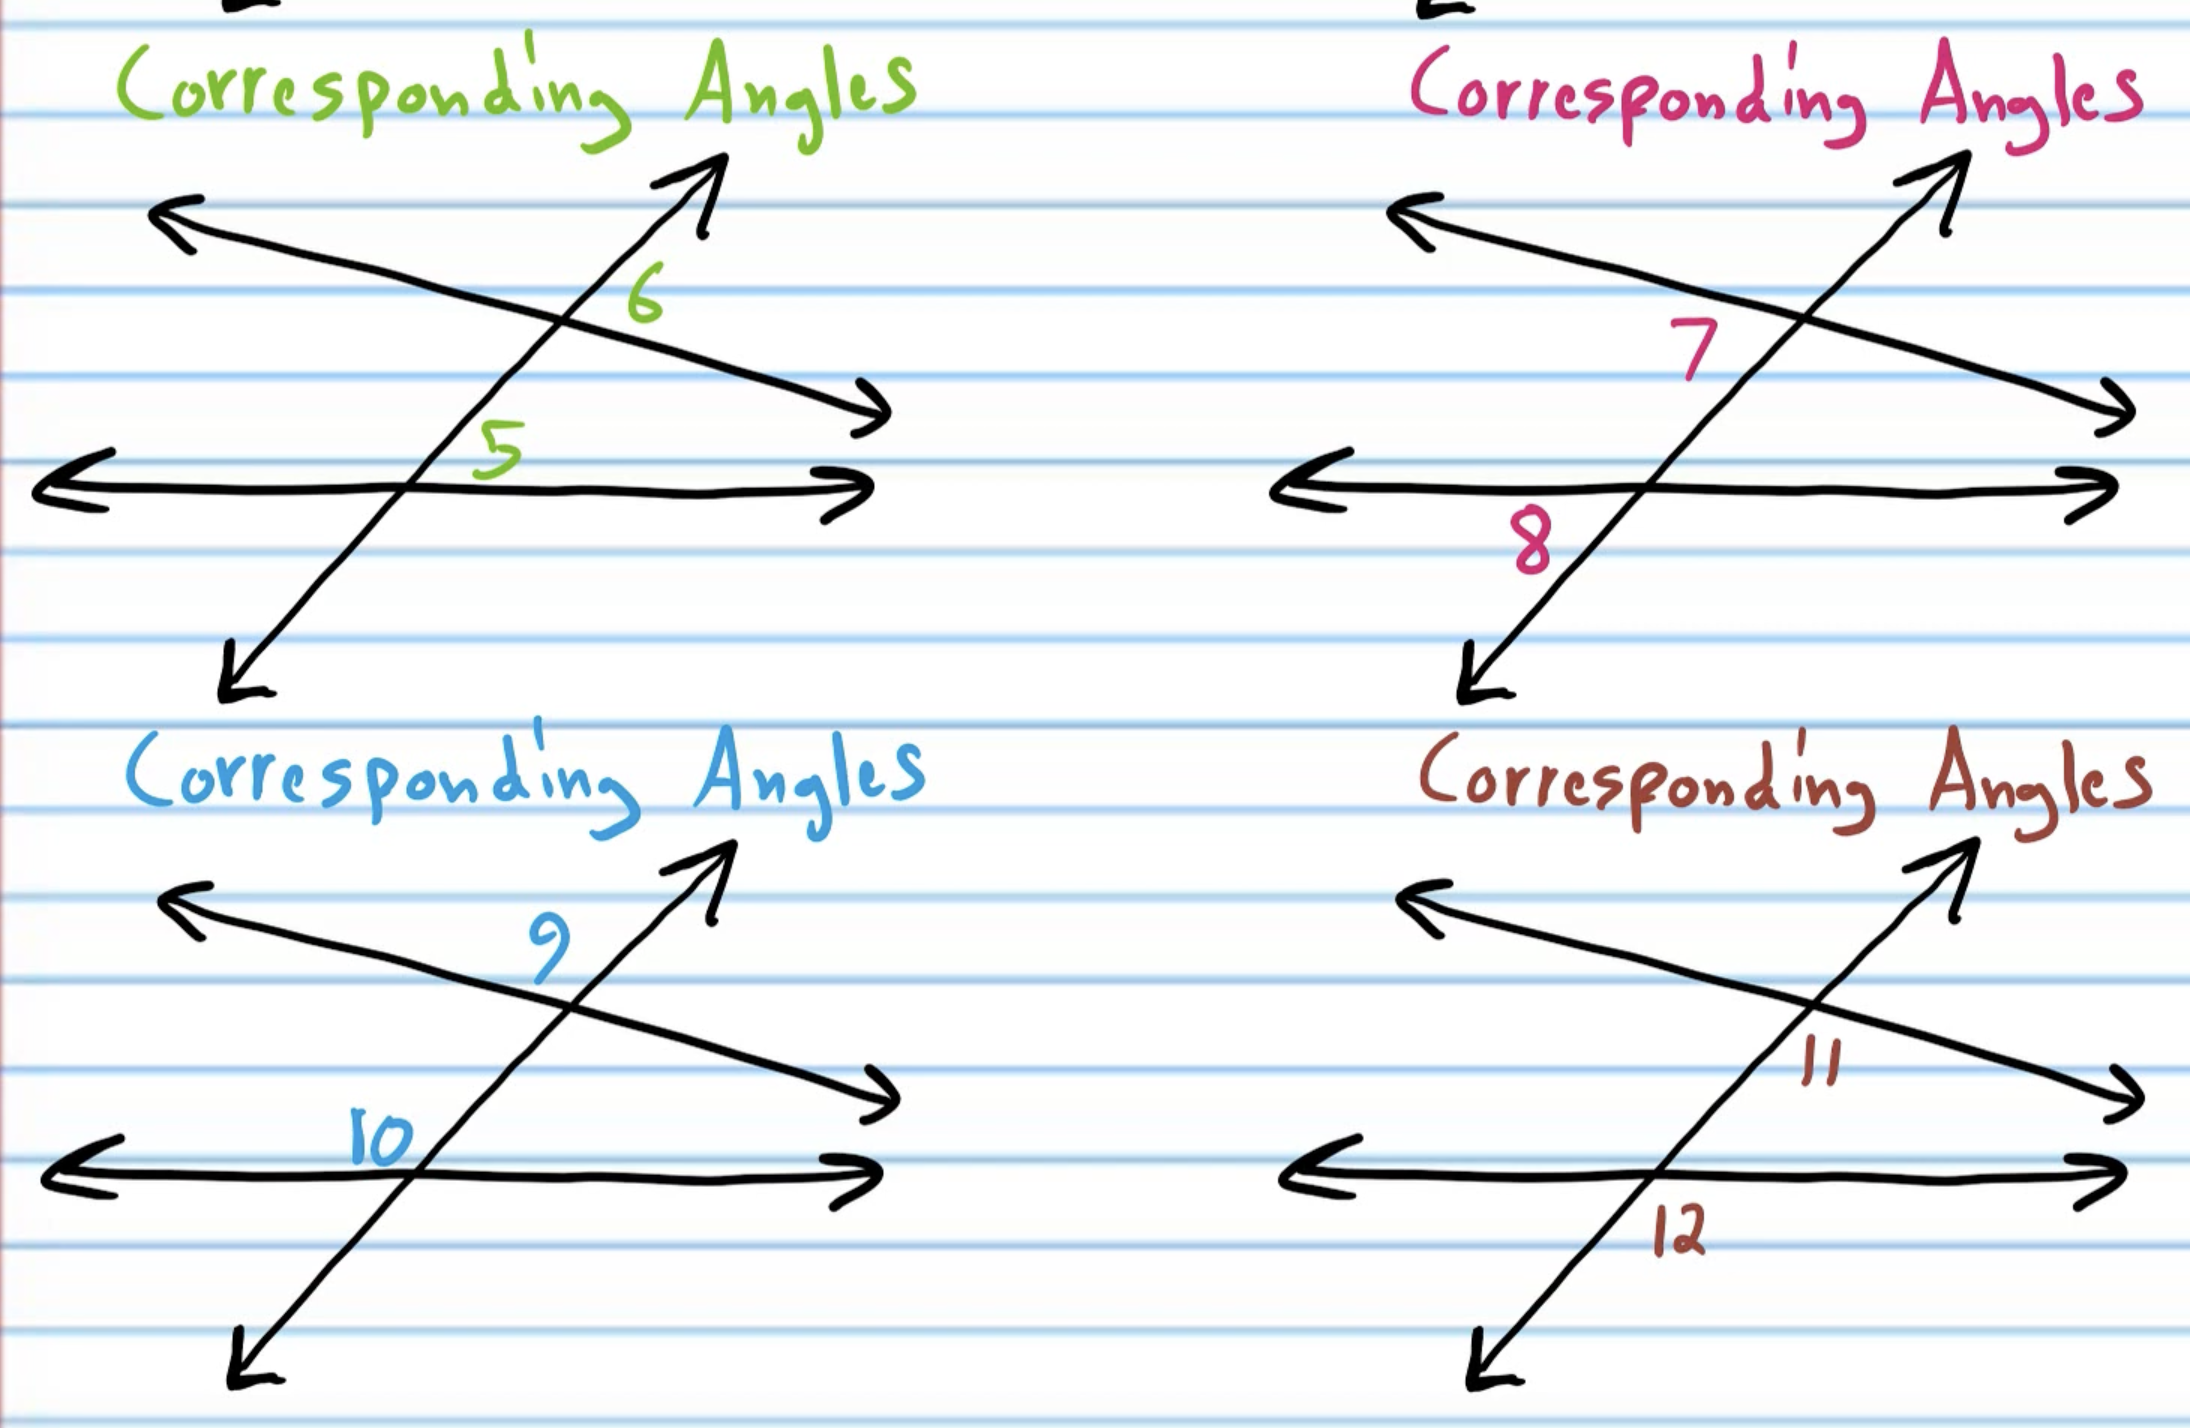
\includegraphics[width=0.8\textwidth]{1102.png}
  \caption{Corresponding Angles}
\end{figure}

\newpage

\begin{figure}[htb!]
  \centering
  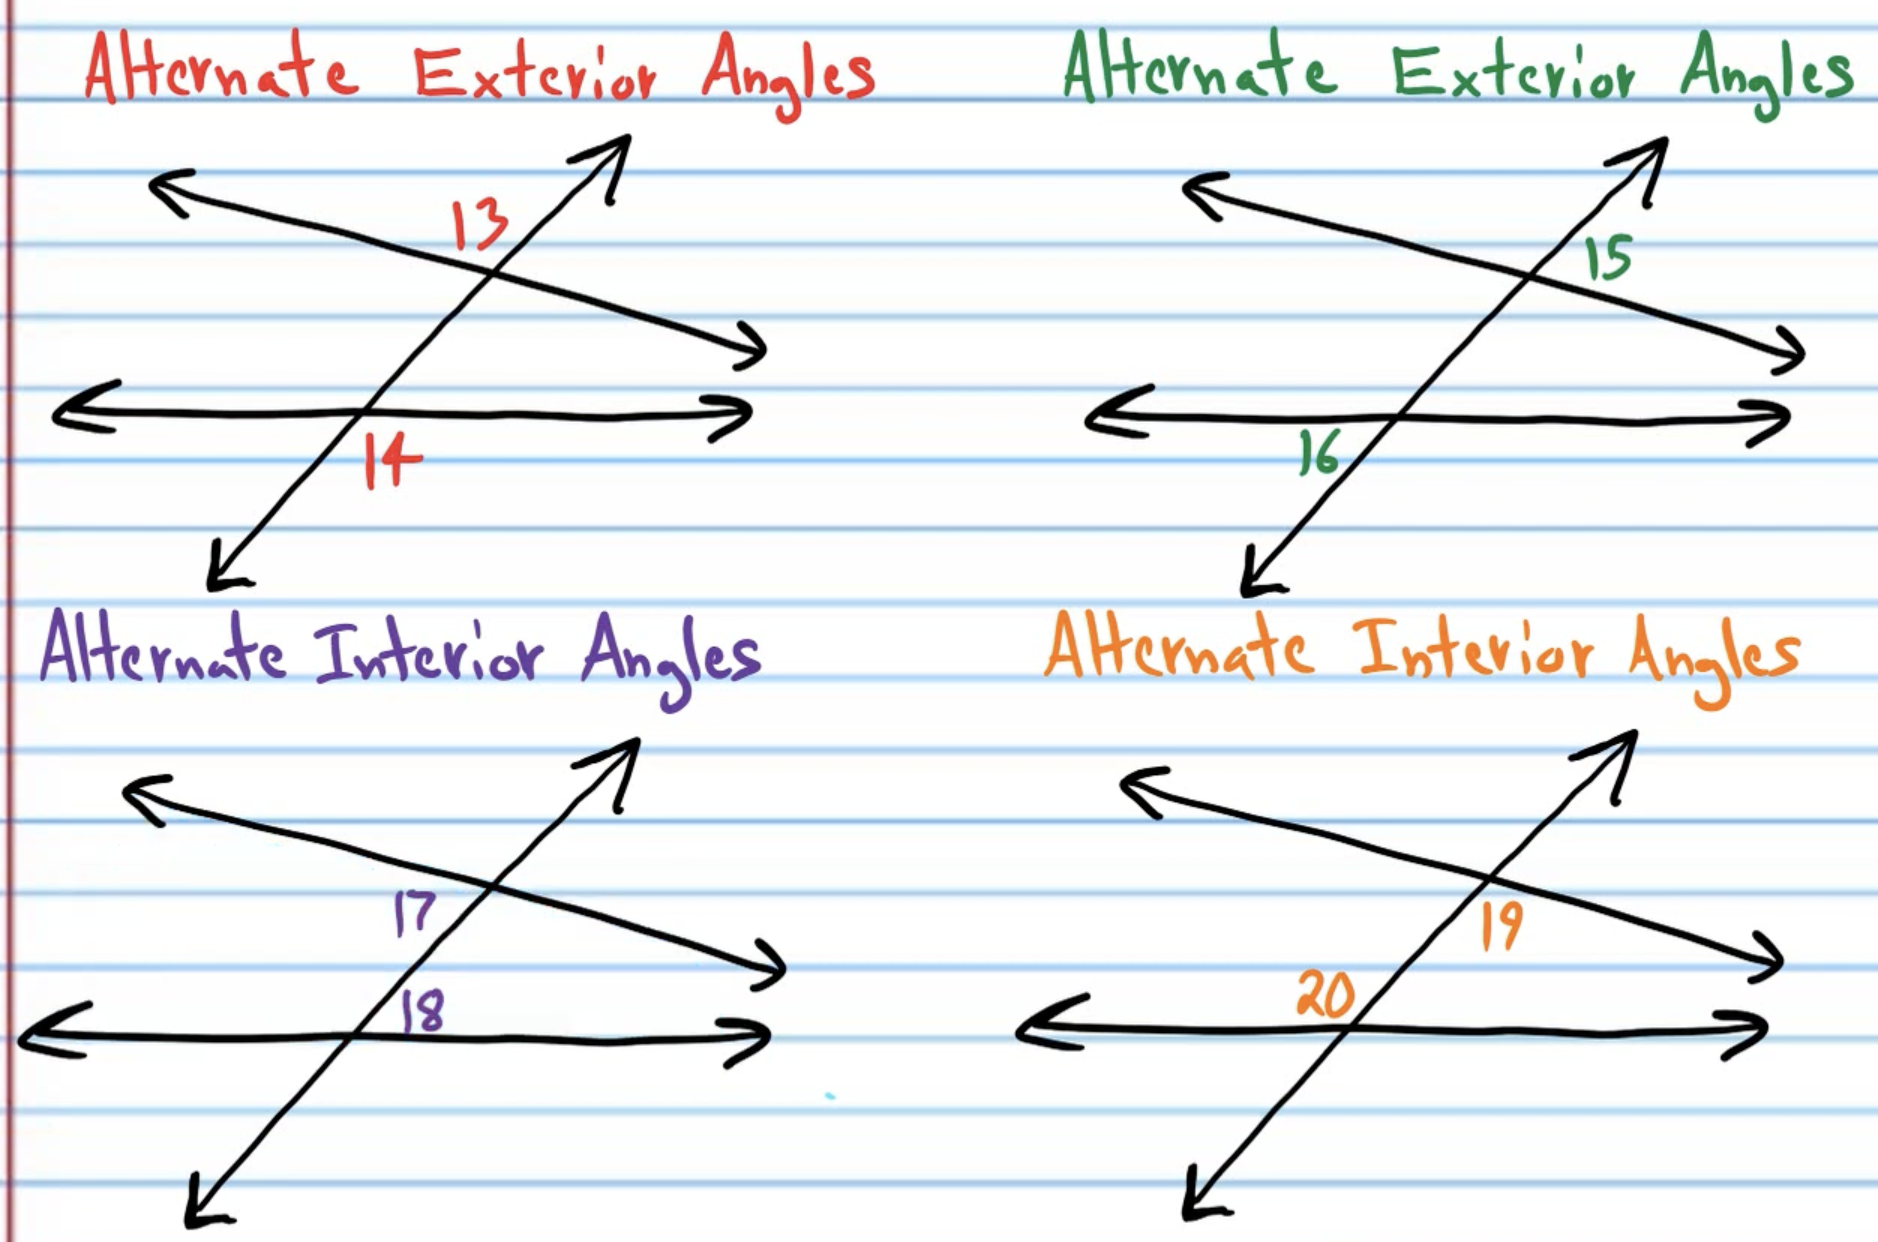
\includegraphics[width=0.8\textwidth]{1103.png}
  \caption{Alternate Angles}
\end{figure}

\begin{figure}[htb!]
  \centering
  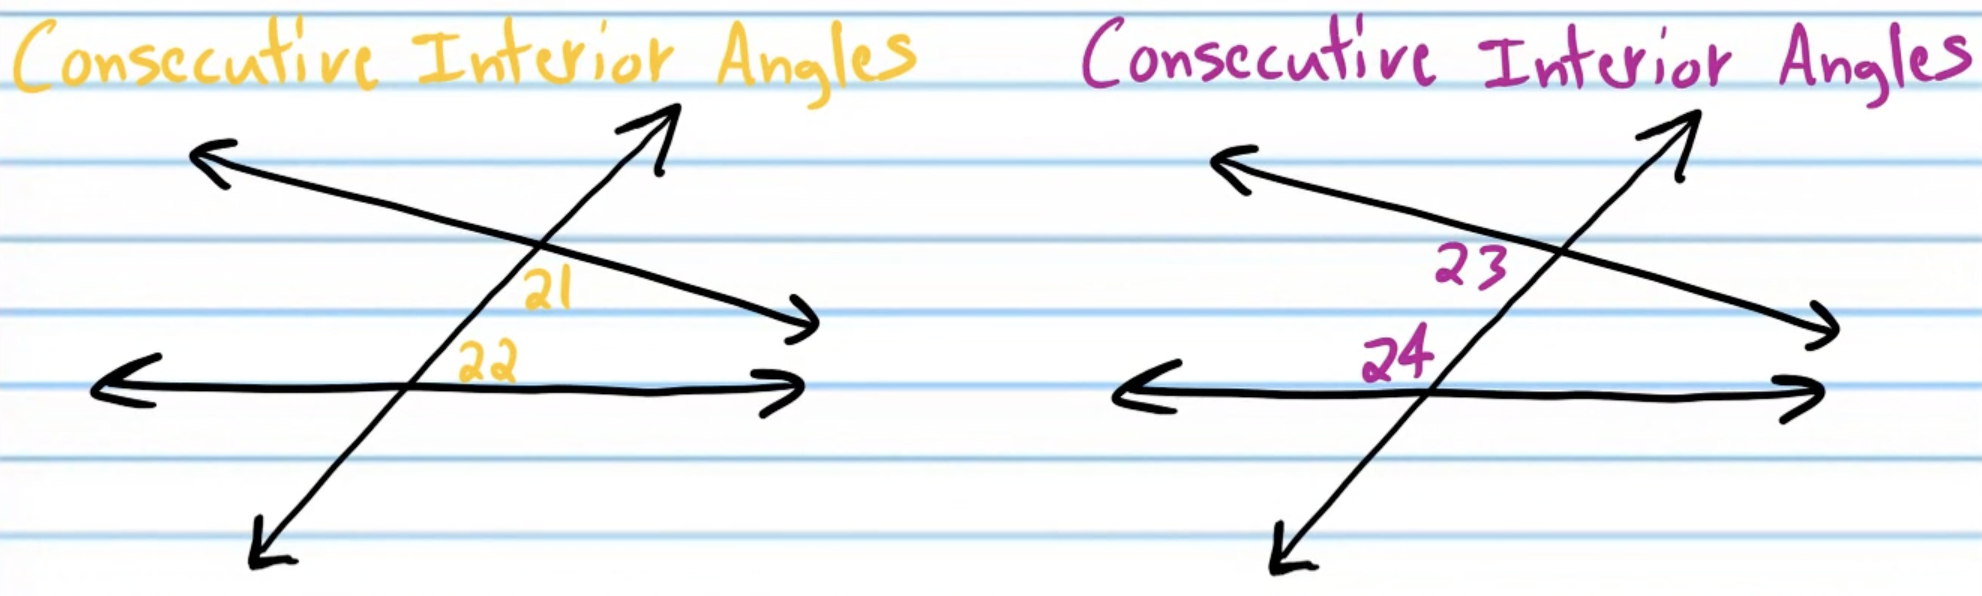
\includegraphics[width=0.8\textwidth]{1104.png}
  \caption{Consecutive Interior Angles}
\end{figure}

\newpage

\centerline{\colorbox{yellow}{\textbf{\underline{\Large Transversals Through Parallel Lines}}}}

\vspace{.5cm}

\begin{tcolorbox}[colback=RoyalPurple!5!white,colframe=RoyalPurple!75!black,title=Corresponding Angles Postulate]
  If parallel lines are cut by a transversal, then corresponding angles formed are congruent.
\end{tcolorbox}

\begin{figure}[htb!]
  \centering
  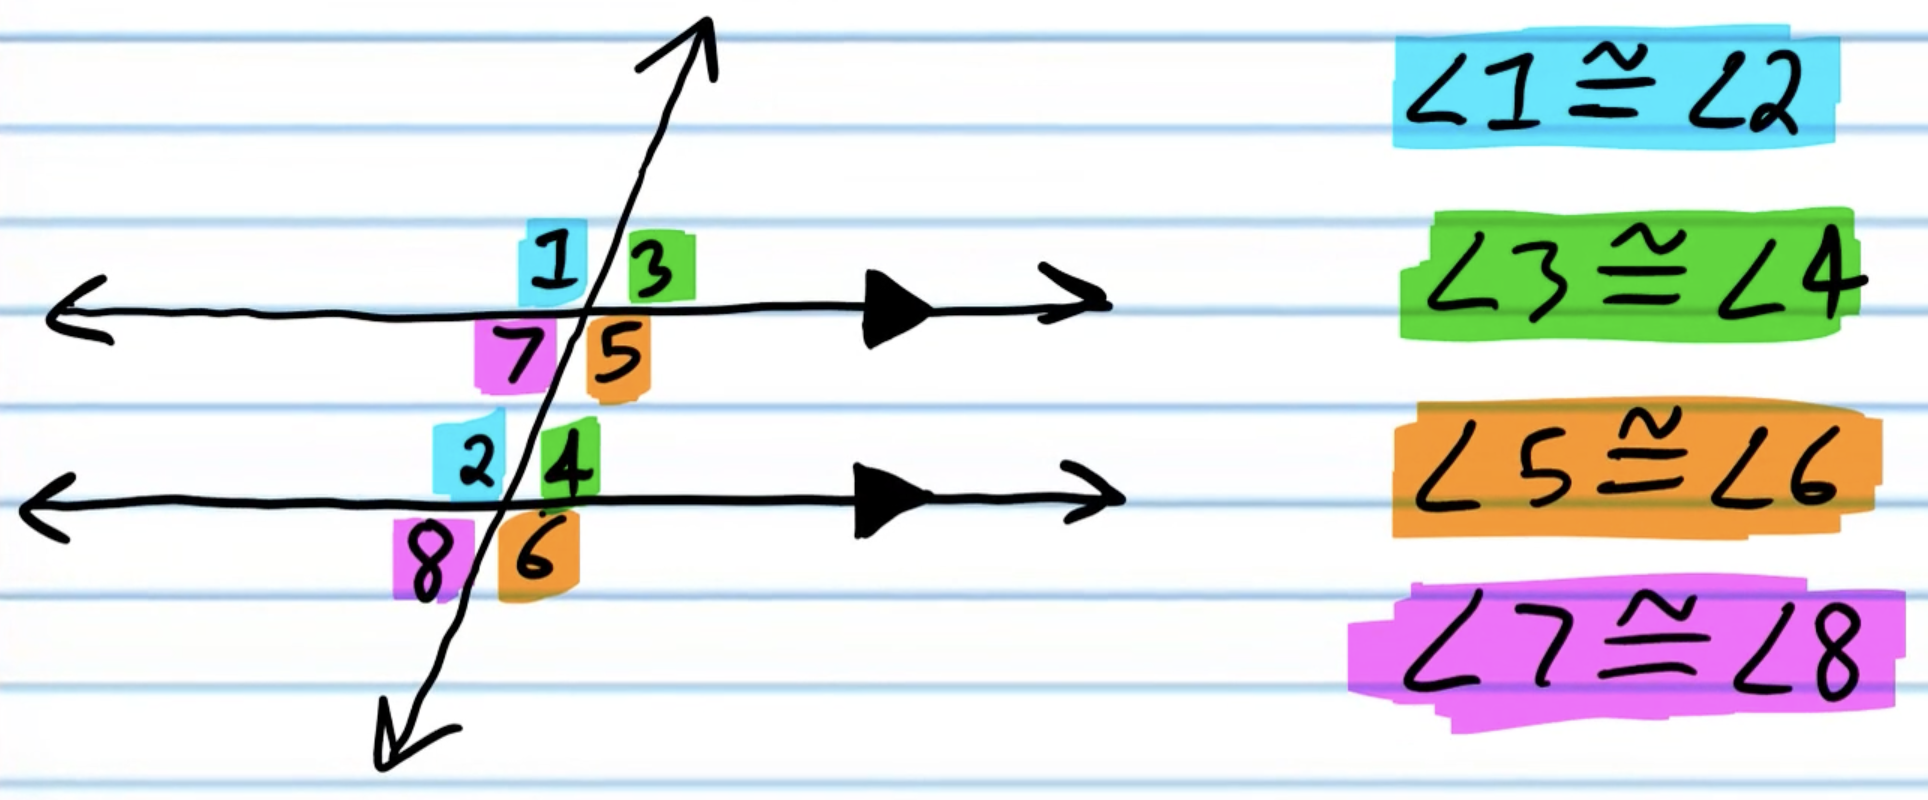
\includegraphics[width=0.7\textwidth]{1105.png}
  \caption{Corresponding Angles Postulate}
\end{figure}

\begin{figure}[htb!]
  \centering
  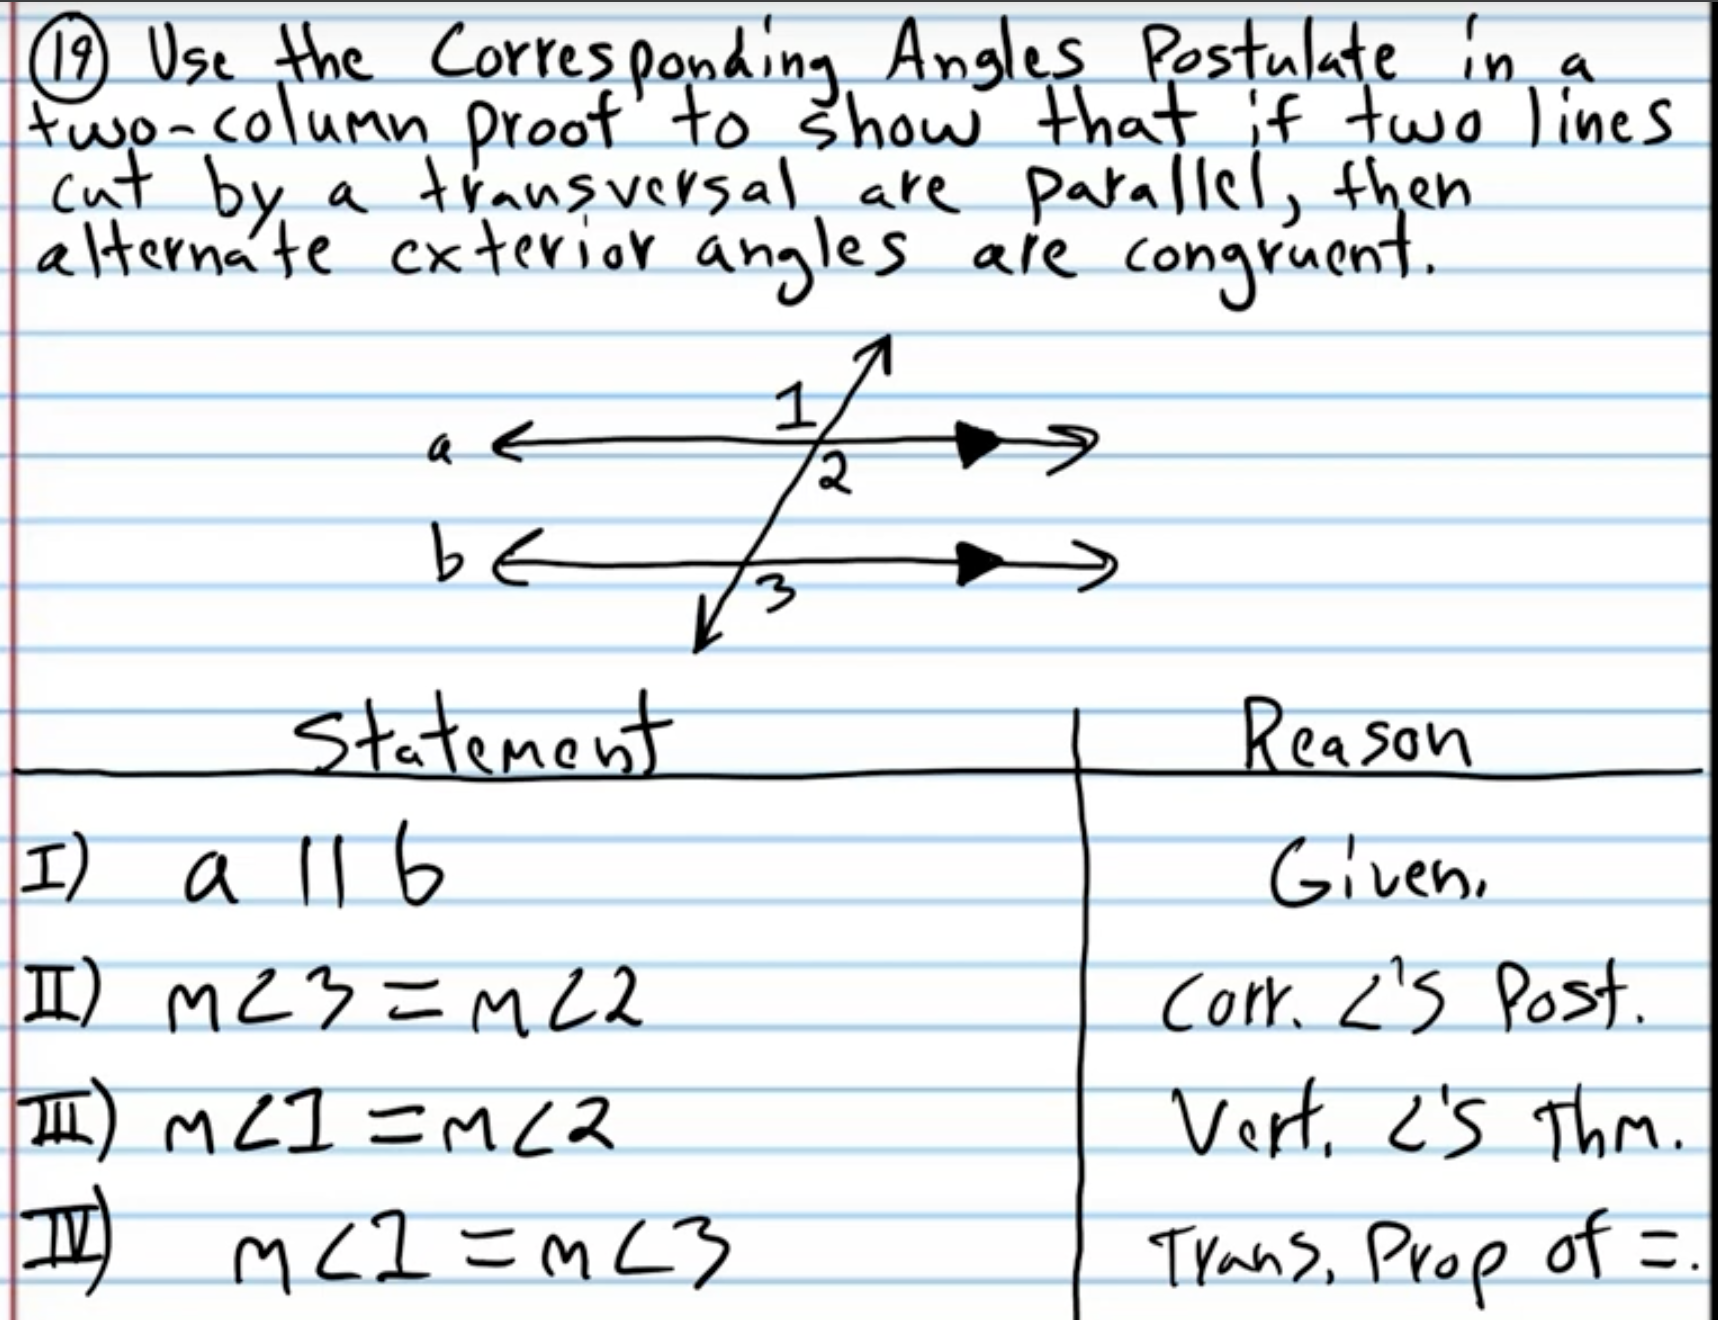
\includegraphics[width=0.8\textwidth]{1106.png}
  \caption{Proving Alternate Exterior Angles Theorem}
\end{figure}

\newpage

\begin{tcolorbox}[colback=Red!5!white,colframe=Red!75!black,title=Alternate Exterior Angles Theorem]
  If parallel lines are cut by a transversal, then alternate exterior angles formed are congruent.
\end{tcolorbox}

\begin{figure}[htb!]
  \centering
  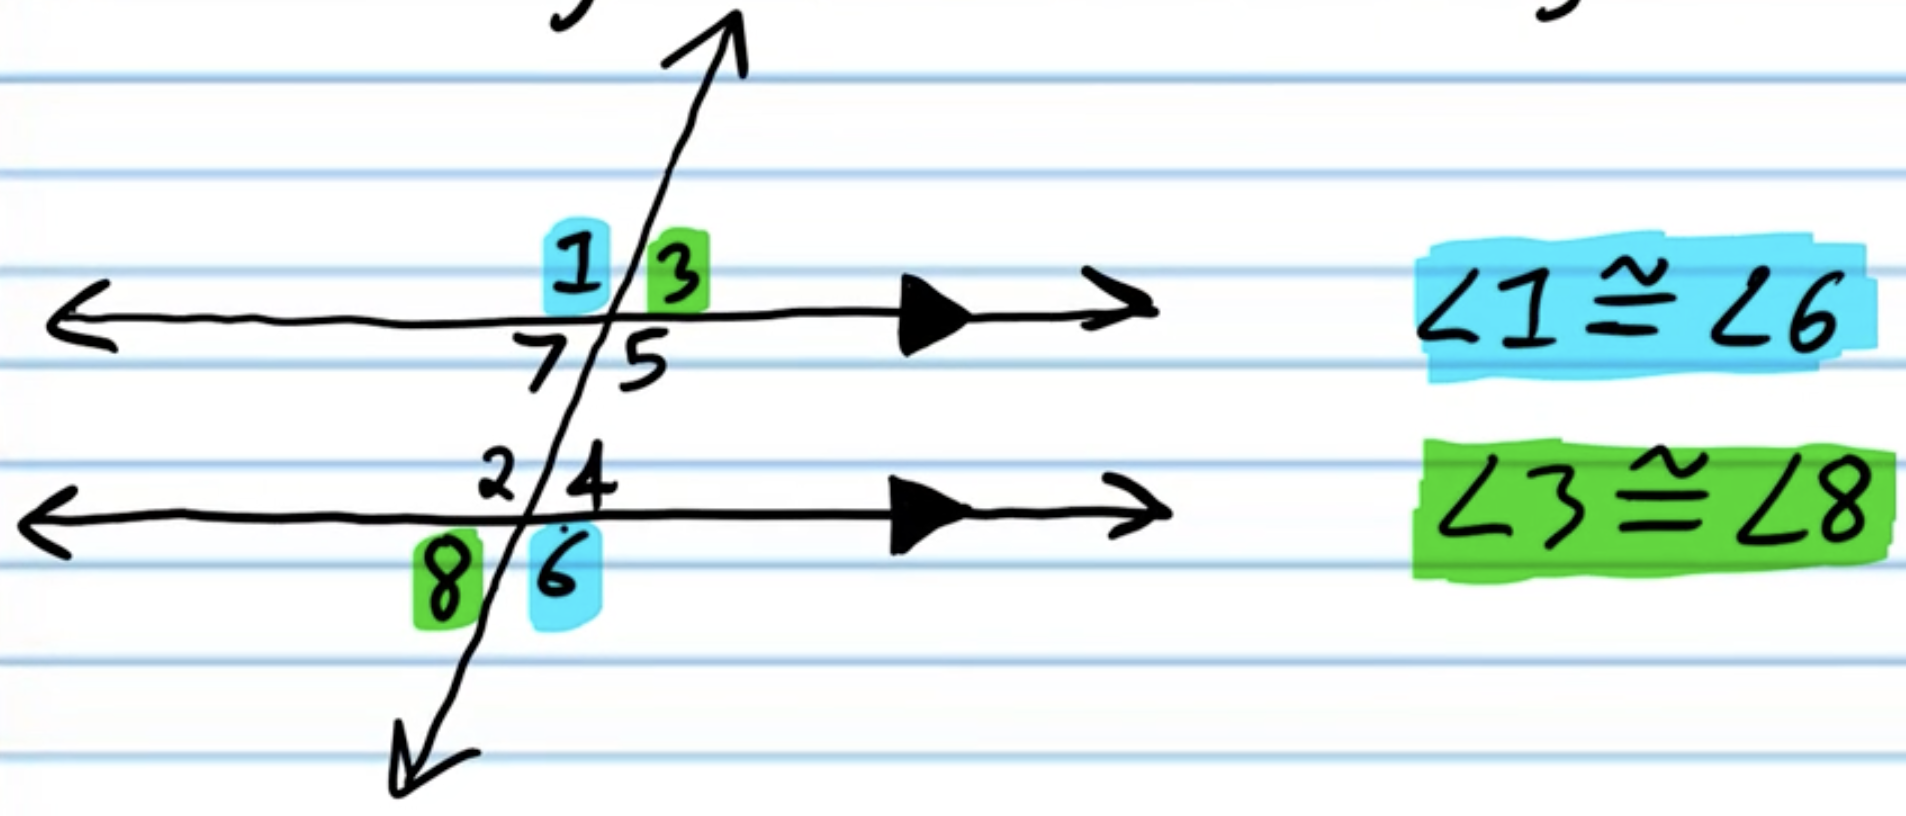
\includegraphics[width=0.8\textwidth]{1107.png}
  \caption{Alternate Exterior Angles Theorem}
\end{figure}

\vspace{.4cm}

\begin{tcolorbox}[colback=Red!5!white,colframe=Red!75!black,title=Alternate Interior Angles Theorem]
  If parallel lines are cut by a transversal, then alternate interior angles formed are congruent.
  % Proof: asset 1108.png
\end{tcolorbox}

\begin{figure}[htb!]
  \centering
  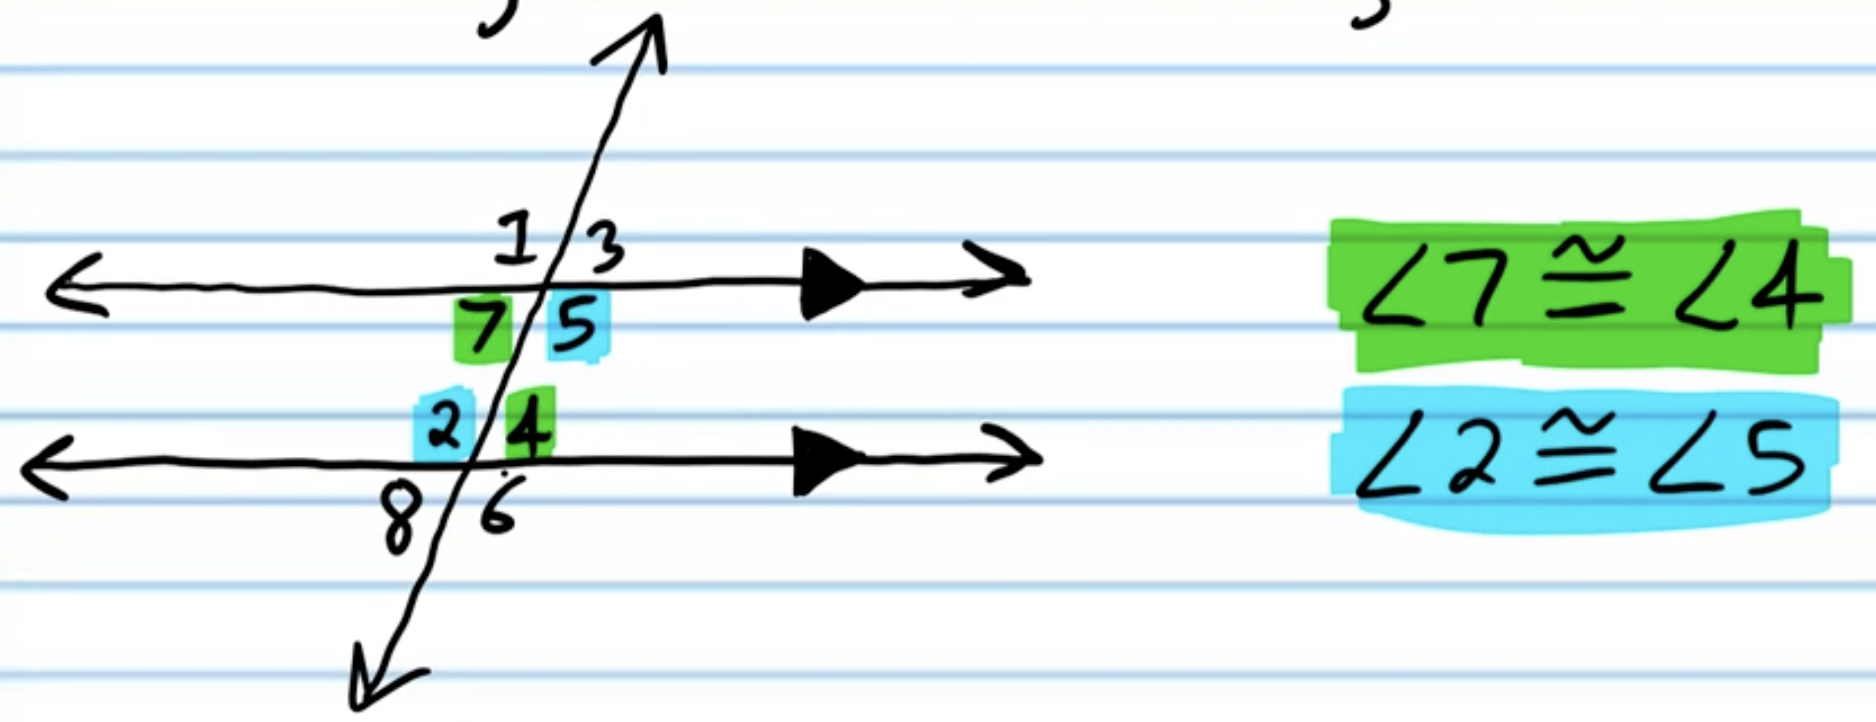
\includegraphics[width=0.8\textwidth]{1109.png}
  \caption{Alternate Interior Angles Theorem}
\end{figure}

\newpage

\begin{tcolorbox}[colback=Red!5!white,colframe=Red!75!black,title=Consecutive Interior Angles Theorem]
  If parallel lines are cut by a transversal, then consecutive interior angles formed are supplementary.
  % Proof: asset 1110.png
\end{tcolorbox}

\begin{figure}[htb!]
  \centering
  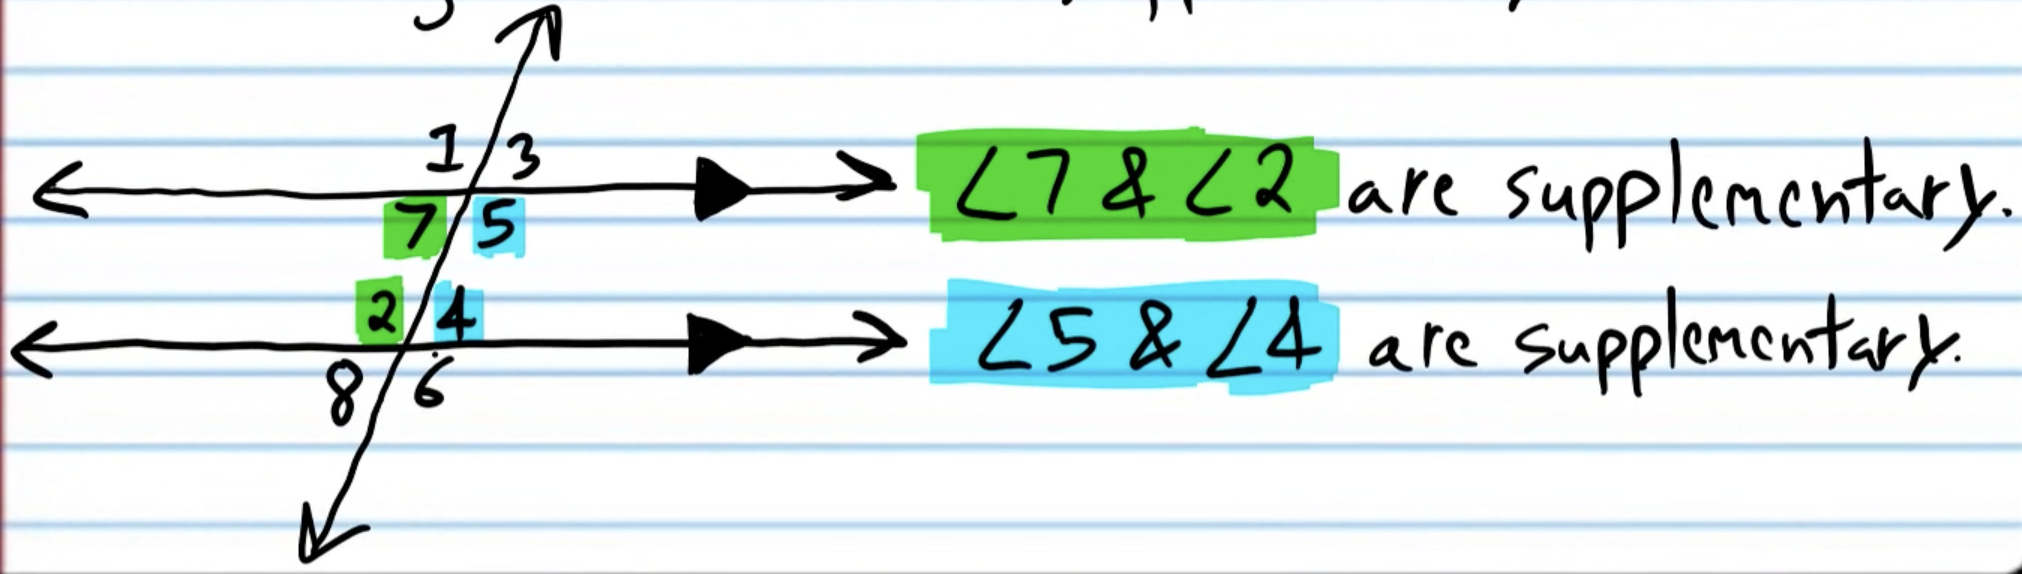
\includegraphics[width=0.8\textwidth]{1111.png}
  \caption{Consecutive Interior Angles Theorem}
\end{figure}

\vspace{.5cm}

\begin{tcolorbox}[colback=RoyalPurple!5!white,colframe=RoyalPurple!75!black,title=Corresponding Angles Converse Postulate]
  If corresponding angles formed by a transversal are congruent, then the lines cut by the transversal are parallel.
\end{tcolorbox}
% Asset 1112.png: use the Postulate above in proof

\threestars
% \vspace{.5cm}

\begin{tcolorbox}[colback=Red!5!white,colframe=Red!75!black,title=Alternate Exterior Angles Converse Theorem]
  If alternate exterior angles formed by a transversal are congruent, then the lines cut by the transversal are parallel.
  % Proof: asset 1113.png
\end{tcolorbox}

\vspace{.2cm}

\begin{tcolorbox}[colback=Red!5!white,colframe=Red!75!black,title=Alternate Interior Angles Converse Theorem]
  If alternate interior angles formed by a transversal are congruent, then the lines cut by the transversal are parallel.
  % Proof: asset 1114.png
\end{tcolorbox}

\vspace{.2cm}

\begin{tcolorbox}[colback=Red!5!white,colframe=Red!75!black,title=Consecutive Interior Angles Converse Theorem]
  If consecutive interior angles formed by a transversal are supplementary, then the lines cut by the transversal are parallel.
  % Proof: asset 1115.png
\end{tcolorbox}

\newpage

\section{Triangles (The Pythagorean Theorem and the Triangle Sum Theorem)}
% 02 Oct 2025 7:30 sáng đi khám sức khỏe nghĩa vụ quân sự

\centerline{\underline{\textbf{\Large Classifying Triangles by}}}

% \vspace{.4cm}

\begin{figure}[htb!]
  \centering
  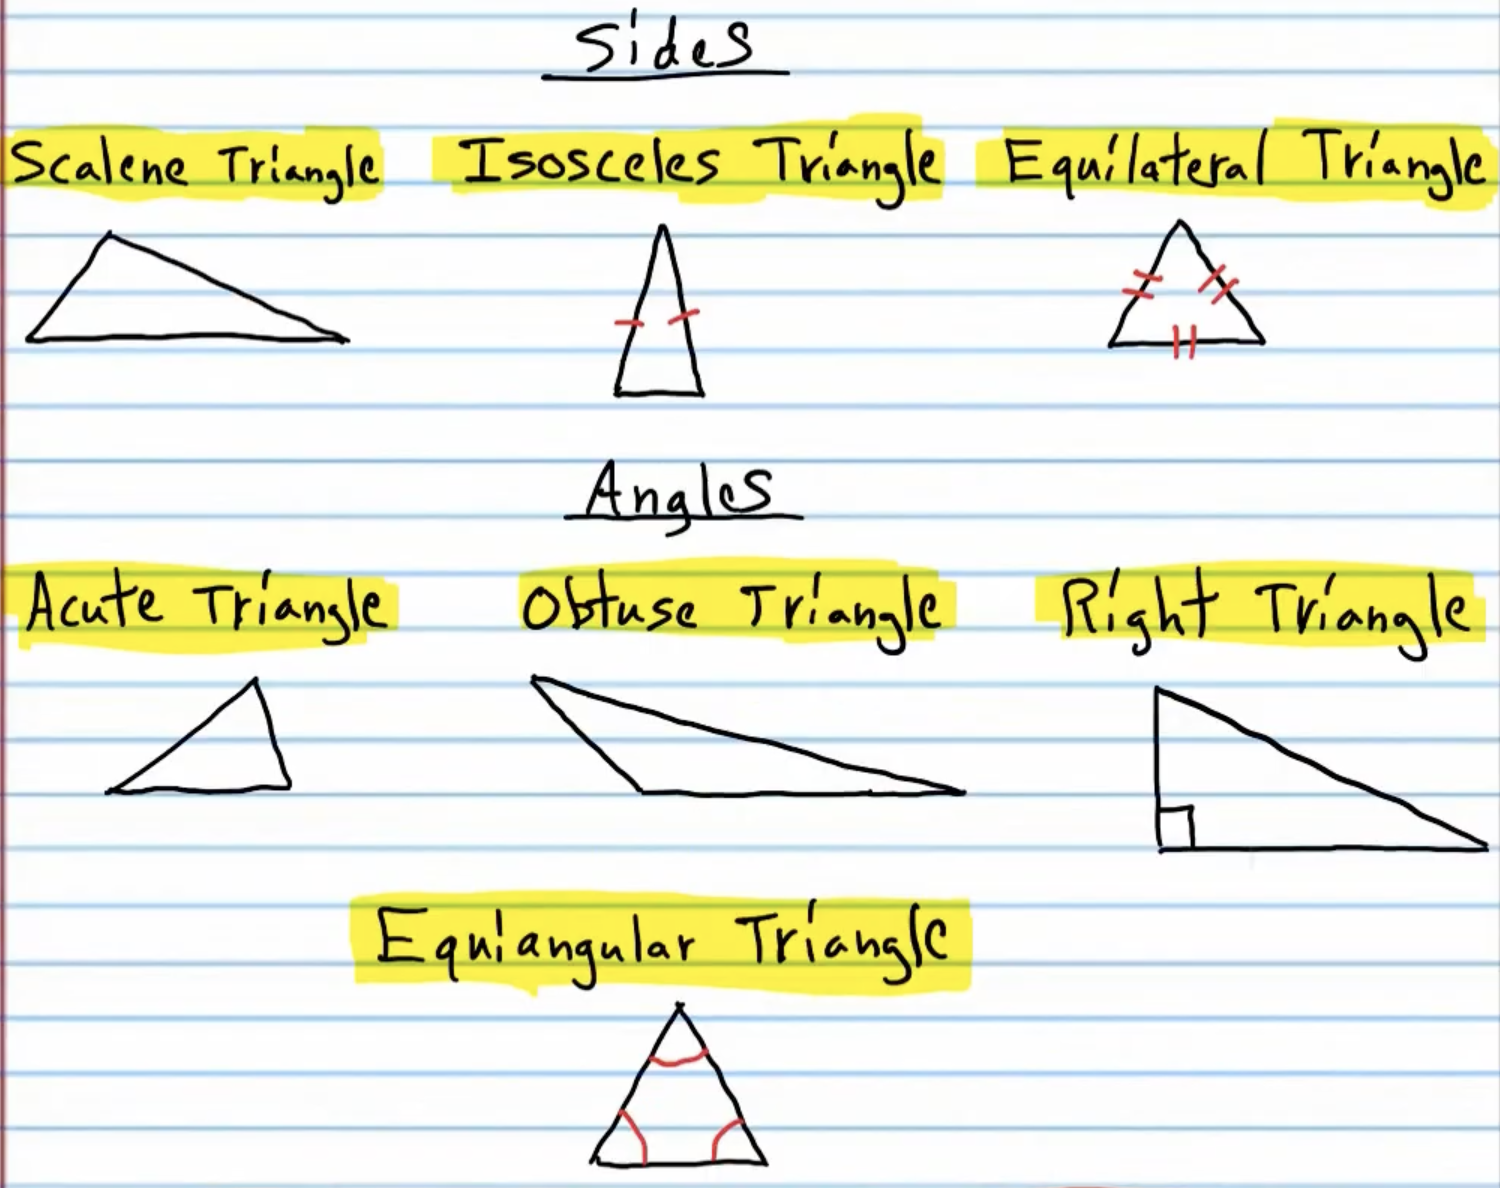
\includegraphics[width=0.8\textwidth]{1201.png}
  \caption{Classifying Triangles}
\end{figure}

In a \hl{Scalene Triangle}, all three side lengths are different.

In an \hl{Acute Triangle}, all three angles are acute angles.

\vspace{.4cm}

\begin{tcolorbox}[colback=Red!5!white,colframe=Red!75!black,title=The Pythagorean Theorem]
  If a, b, and c are the legs and hypotenuse of a right triangle, respectively, then $a^{2}+b^{2}=c^{2}$.
\end{tcolorbox}

\begin{figure}[htb!]
  \centering
  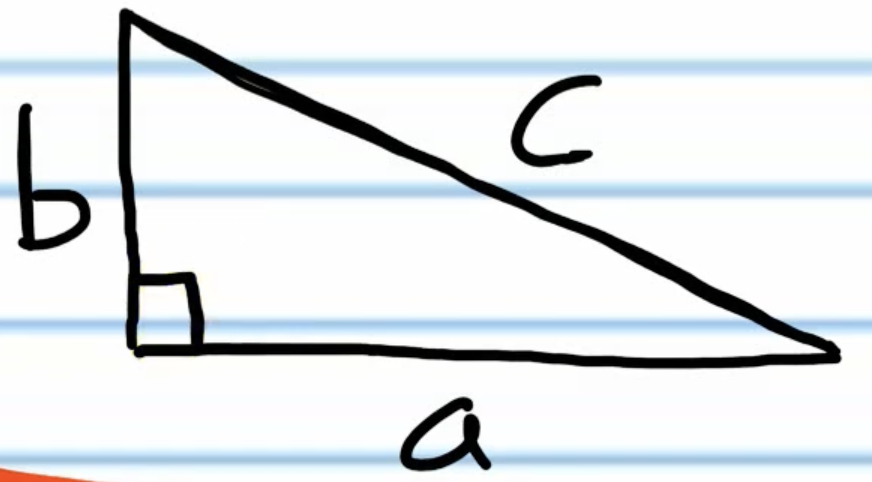
\includegraphics[width=0.26\textwidth]{1202.png}
  \caption{The Pythagorean Theorem}
\end{figure}

\newpage

When working with the Pythagorean equation, the correct answers algebraically when you square root both sides have ($\pm$) sign. But triangle length cannot be negative, so we ignore the negative answer.

\vspace{.5cm}

\begin{figure}[htb!]
  \centering
  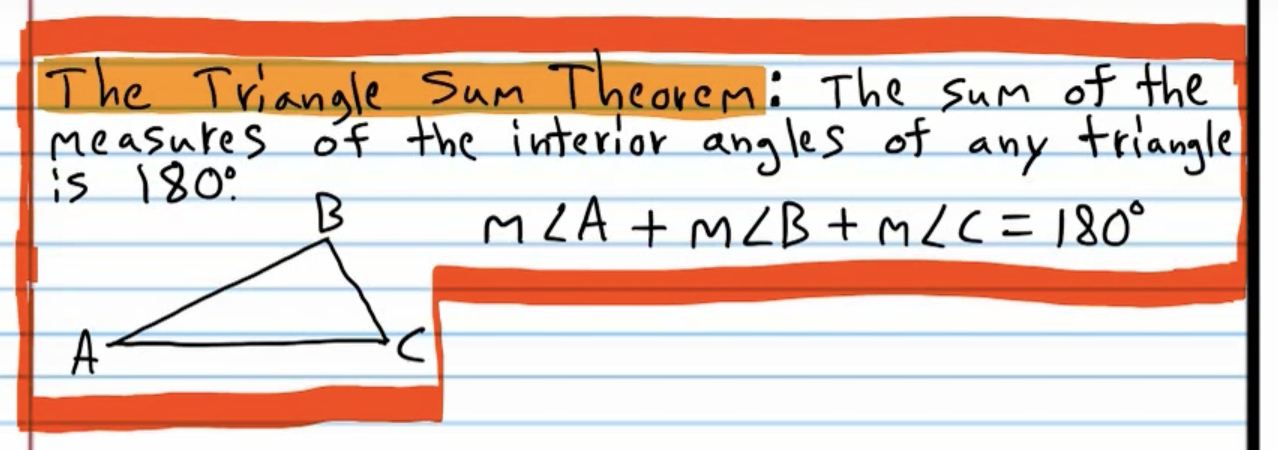
\includegraphics[width=1\textwidth]{1203.png}
  \caption{The Triangle Sum Theorem}
\end{figure}

% \vspace{.3cm}

\begin{tcolorbox}[colback=Red!5!white,colframe=Red!75!black,title=Right Triangle Complements Theorem (unimportant)]
  The two acute angles in a right triangle are complementary.
  % Proof: asset 1205.png
\end{tcolorbox}

\begin{figure}[htb!]
  \centering
  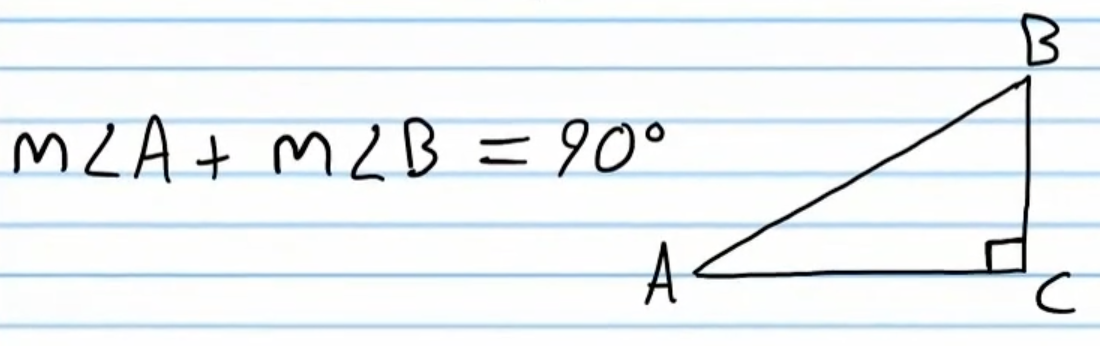
\includegraphics[width=.57\textwidth]{1204.png}
  \caption{Right Triangle Complements Theorem}
\end{figure}

\begin{tcolorbox}[colback=Red!5!white,colframe=Red!75!black,title=Exterior Angle Theorem (unimportant)]
  The measure of an exterior angle of a triangle is equal to the sum of the measures of the two nonadjacent interior angles.
  % Proof: asset 1207.png
\end{tcolorbox}

\begin{figure}[htb!]
  \centering
  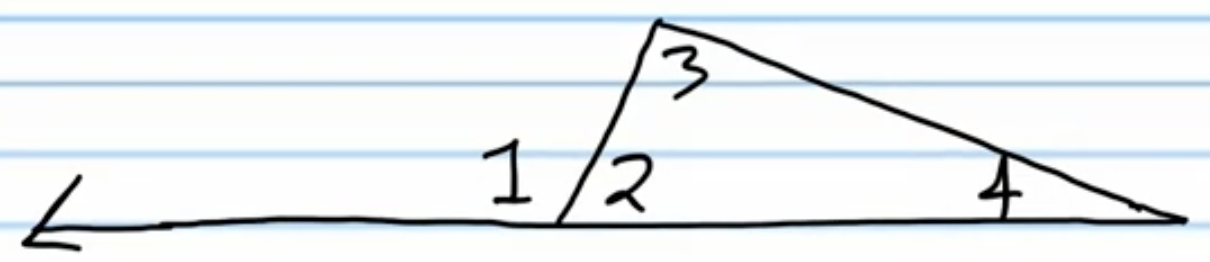
\includegraphics[width=.57\textwidth]{1206.png}
  \caption{Exterior Angle Theorem}
\end{figure}

\newpage

\begin{tcolorbox}[colback=Red!5!white,colframe=Red!75!black,title=Third Angles Theorem (unimportant)]
  If the measures of two angles in one triangle are equal to the measures of two angles in another triangle, then the measures of the third angles in the triangles are equal.
  % Proof: asset 1209.png
\end{tcolorbox}

\begin{figure}[htb!]
  \centering
  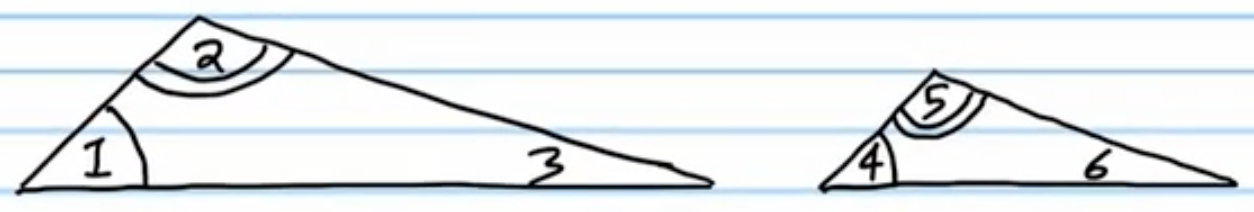
\includegraphics[width=.6\textwidth]{1208.png}
  \caption{Third Angles Theorem}
\end{figure}

\section{Triangle Congruence Postulates and Theorems}
% k

\hl{Congruent Polygons}: Polygons are congruent if they have the same size and shape. More specifically, they are congruent if corresponding angles are congruent and corresponding sides are congruent.

\begin{figure}[htb!]
  \centering
  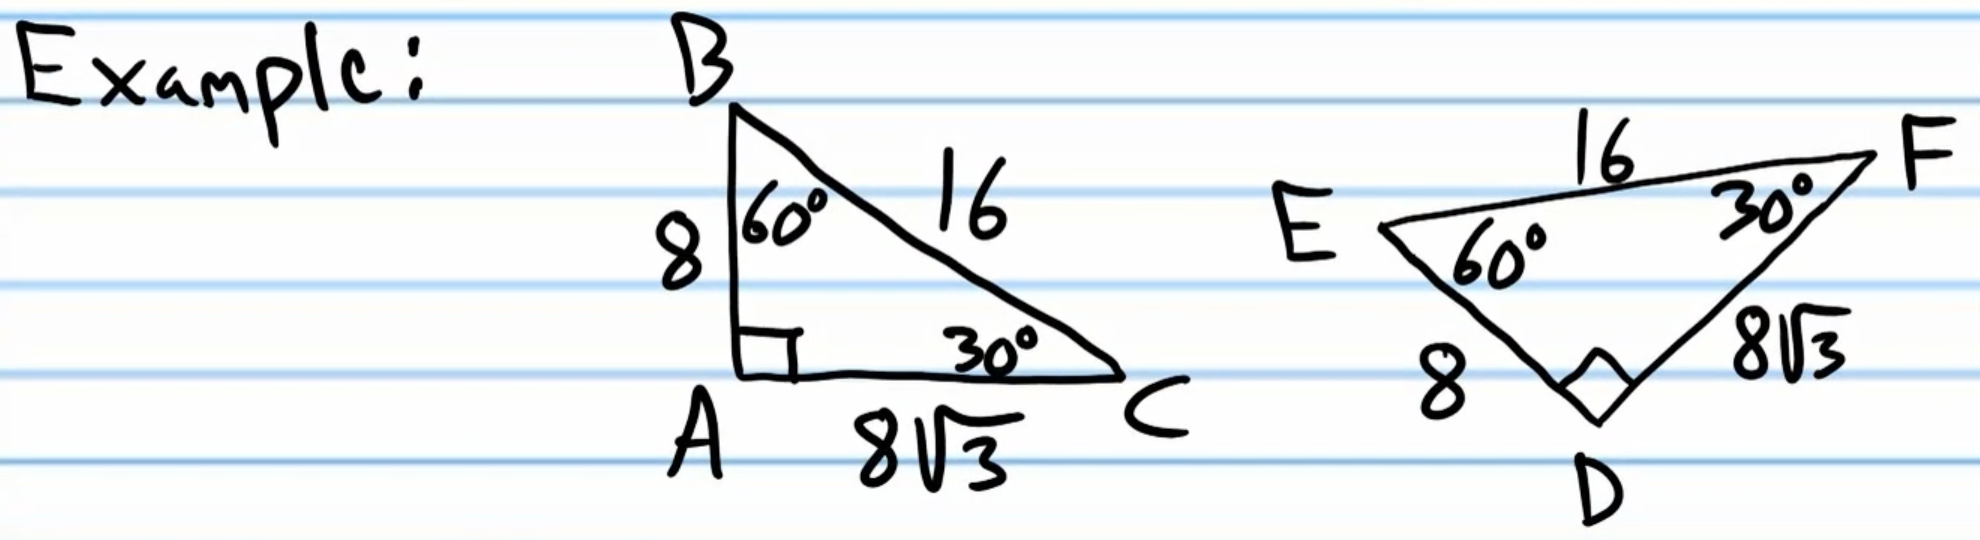
\includegraphics[width=.7\textwidth]{1301.png}
  \caption{Congruent Polygons}
\end{figure}

\begin{figure}[htb!]
  \centering
  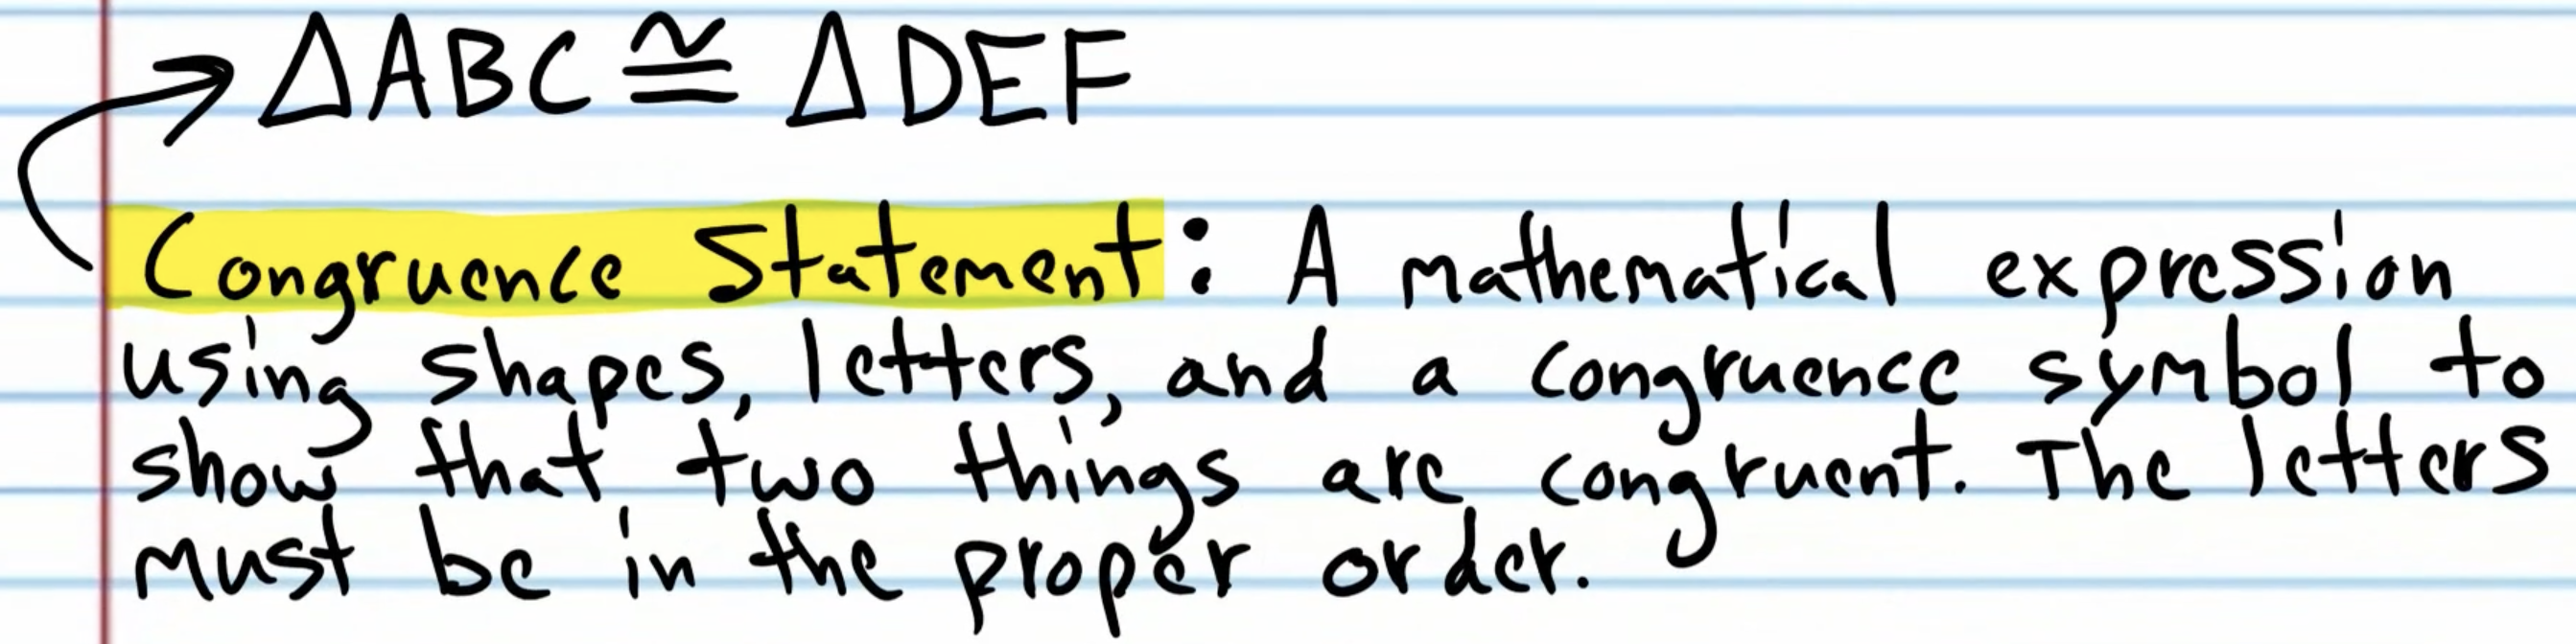
\includegraphics[width=1\textwidth]{1302.png}
  \caption{Congruent Statements}
\end{figure}

\newpage

\centerline{\underline{\hl{\textbf{\huge Triangle Congruence}}}}

\vspace{.5cm}

\begin{tcolorbox}[colback=Red!5!white,colframe=Red!75!black,title=Side-Side-Side Congruence Postulate]
  If each side in one triangle is congruent to each corresponding side in another triangle, then the triangles are congruent. This postulate is abbreviated SSS.
\end{tcolorbox}

\begin{figure}[htb!]
  \centering
  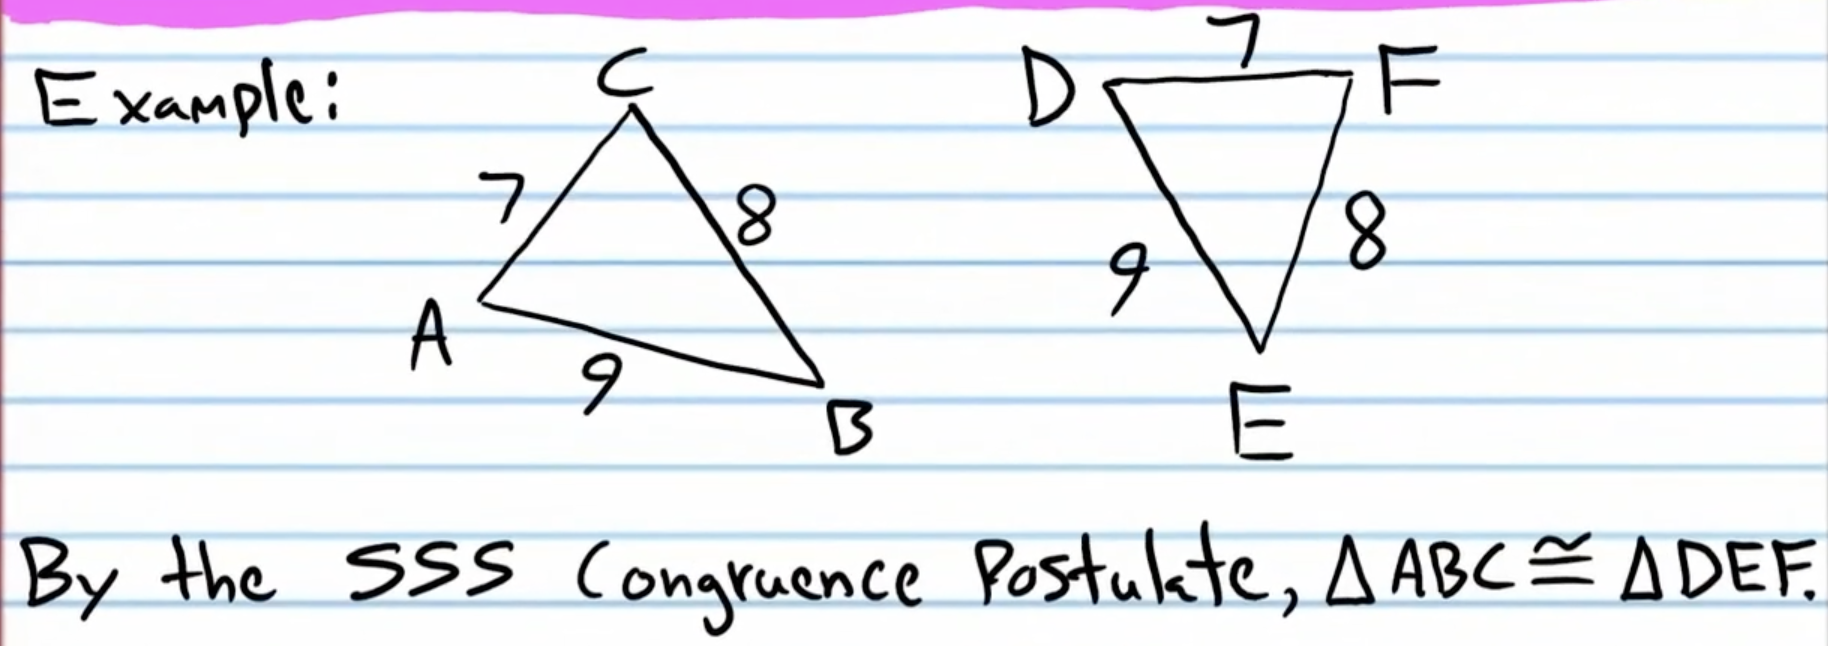
\includegraphics[width=.7\textwidth]{1303.png}
  \caption{Side-Side-Side Congruence Postulate}
\end{figure}

\begin{tcolorbox}[colback=Red!5!white,colframe=Red!75!black,title=Side-Angle-Side Congruence Postulate]
  If two sides and the included angle in one triangle are congruent to two sides and the included angle in another triangle, then the triangles are congruent. This postulate is abbreviated SAS.
\end{tcolorbox}

\begin{figure}[htb!]
  \centering
  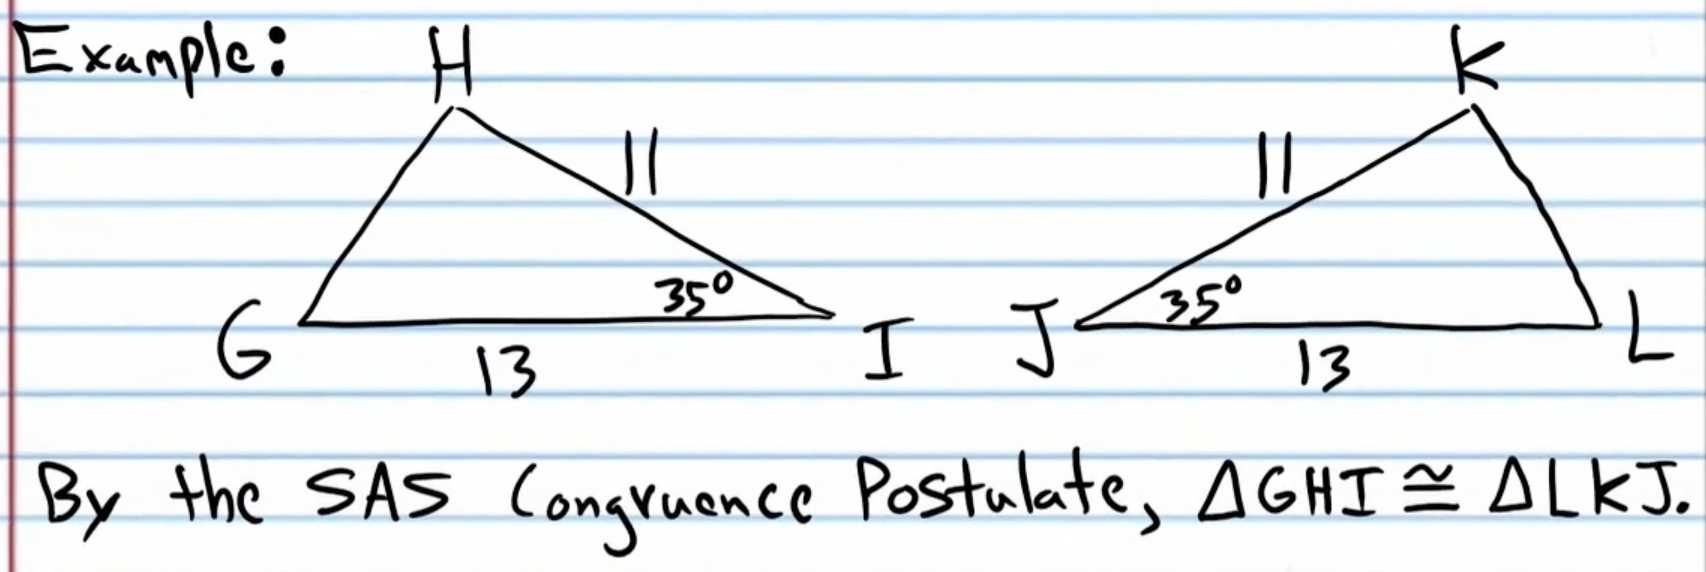
\includegraphics[width=.7\textwidth]{1304.png}
  \caption{Side-Angle-Side Congruence Postulate}
\end{figure}

